\documentclass{standalone}
\usepackage[english]{babel}
% https://tex.stackexchange.com/questions/570303/use-blacktriangleright-as-itemize-label

\usepackage{amssymb} % for black triangleright

\usepackage{amsmath}

\usepackage{graphicx}
% \graphicspath{figures/}

\renewcommand{\labelitemi}{$\textcolor{SwitchColor}{\bullet}$}
\renewcommand{\labelitemii}{$\textcolor{SwitchColor}{\blacktriangleright}$}
\renewcommand{\labelitemiii}{$\textcolor{SwitchColor}{\blacksquare}$}

% https://tex.stackexchange.com/questions/525959/prevent-latex-from-stretching-math
\setlength{\thinmuskip}{1\thinmuskip}
\setlength{\medmuskip}{1\medmuskip}
\setlength{\thickmuskip}{1\thickmuskip}

\usepackage{etoolbox}

\usepackage{mathtools}

\newtoggle{absolute}
% \toggletrue{absolute}
\togglefalse{absolute}

\newcommand{\lpathgraph}[1]{\iftoggle{absolute}{/home/areo/Documents/Studium/Summaries/Graph_Theory/}{./}#1}
\newcommand{\lpathsearch}{\iftoggle{absolute}{/home/areo/Documents/Studium/Summaries/Search_Algorithms/main.pdf}{./Search_Algorithms.pdf}}
\newcommand{\lpathdfssearch}{\iftoggle{absolute}{/home/areo/Documents/Studium/Summaries/Search_Algorithms/AD_Vorlesung08_with_go_back.pdf}{./AD_Vorlesung08_with_go_back.pdf}}

\usepackage[style=numeric]{biblatex}
\addbibresource{./Graph_Theory.bib}

\usepackage{csquotes}
\usepackage{xcolor}
% \usepackage{anyfontsize}
\usepackage[export]{adjustbox}
% \usepackage[]{enumitem}
\usepackage{tikz}
\usetikzlibrary{arrows.meta,positioning}
\usetikzlibrary{graphs}
\usetikzlibrary{patterns}
\usetikzlibrary{shadings}
\usetikzlibrary{mindmap, shadows, backgrounds} % , calc

\definecolor{SecondaryColor}{HTML}{BBAF01}
\definecolor{SecondaryColorDimmed}{HTML}{FEF684}
\definecolor{PrimaryColor}{HTML}{E95112}
\definecolor{PrimaryColorDimmed}{HTML}{F6AF91}
\definecolor{SwitchColor}{named}{PrimaryColor}
\colorlet{BoxColor}{gray!10!white}

\usepackage[allbordercolors=PrimaryColor, pdfborder={0 0 .2}]{hyperref}

% colored bold
% \newcommand\alert[1]{\textcolor{SwitchColor}{\textbf{#1}}}
\newcommand\alert[1]{\textcolor{SwitchColor}{#1}}

\newlength{\leveldistance}
\setlength{\leveldistance}{25cm}

% to input other file start
\usepackage{pseudo}
\usepackage{xparse}
\usepackage{tcolorbox}
\tcbuselibrary{skins,theorems}

\newcounter{algorithm}
\setcounter{algorithm}{0}
\newtcbtheorem[use counter=algorithm]{algorithm}{\color{SecondaryColor}Algorithm}{pseudo/ruled}{alg}

\newcommand{\ma}[1]{$\mathcal{#1}$}
\renewcommand{\tt}[1]{{\small\texttt{#1}}}

% https://tex.stackexchange.com/questions/600708/input-inside-tikzpicture-differs-from-inserting-manually
\ExplSyntaxOn
\cs_new:Npn \expandableinput #1
  { \use:c { @@input } { \file_full_name:n {#1} } }
\AddToHook{env/tikzpicture/begin}
  { \cs_set_eq:NN \input \expandableinput }
\ExplSyntaxOff

\usepackage{fontspec}
\newfontfamily\gyre{DejaVu Math TeX Gyre}

%!Tex Root = ../main.tex

\NewDocumentCommand{\bfs}{s}{
  \begin{algorithm}{\pr{Breadth-First Search as Graph-Search}($G$, $s$, $t$)}{\thetcbcounter}
    \begin{pseudo}[indent-mark,kw,hl-warn=false]
      \ma{Q} $\leftarrow$ \tt{new.Queue()}\\
      \tt{counter} $\leftarrow 1$\\
      \ma{Q}\tt{.enqueue($s$)}; \tn{mark $s$}\\
      \tt{s.count} $\leftarrow$ \tt{counter}; \tt{counter} $\leftarrow$ \tt{counter} $+ 1$ \\
      As long as \tn{not \ma{Q}.empty()} do\\+
        $u \leftarrow$ \ma{Q}\tt{.dequeue()}\IfBooleanTF#1{\\[hl]}{\\} 
        if $u$ is $t$ then\IfBooleanTF#1{\\+[hl]}{\\+} 
          return \cn{true}\\-
        for each \tn{adjavent node $v$ of $u$ in $G$} do\\+
          if $v$ \tn{not marked} then\\+
            \ma{Q}\tt{.enqueue($v$)}; \tn{mark $v$}\\
            $v$\tt{.count} $\leftarrow$ \tt{counter}; \tt{counter} $\leftarrow$ \tt{counter} $+ 1$ \IfBooleanTF#1{\\---[hl]}{\\---}
      return \cn{false}
    \end{pseudo}
  \end{algorithm}
}

\NewDocumentCommand{\dfs}{s}{
  \begin{algorithm}{\pr{Depth-First Search as Graph Search}($G$, $s$, $t$)}{\thetcbcounter}
    \begin{pseudo}[indent-mark,kw,hpad=0.6cm]
      \ma{S} $\leftarrow$ \tt{new.Stack()} \\
      \tt{counter} $\leftarrow 1$\\
      \ma{S}\tt{.push($s$);} \tn{mark} $s$\\
      $s$\tt{.start} $\leftarrow$ \tt{counter;} \tt{counter} $\leftarrow$ \tt{counter} $+ 1$\IfBooleanTF#1{\\[hl]}{\\}
      if $s$ is $t$ then\IfBooleanTF#1{\\+[hl]}{\\+}
        return \cn{true}\\-
      As long as \tn{not \ma{S}\tt{.empty()}} do\\+
        % $u \leftarrow$ \ma{S}\tt{.pop();} \ma{S}\tt{.push($u$)}\\
        $u \leftarrow$ \ma{S}\tt{.look\_at\_top()}\\
        if \tn{a not marked adjacent node $v$ of $u$ exists in $G$} then\\+
          \ma{S}\tt{.push($v$);} \tn{mark} $v$\IfBooleanTF#1{\\[hl]}{\\}
          if $v$ \tn{is} $t$ then\IfBooleanTF#1{\\+[hl]}{\\+}
            return \cn{true}\\-
          $v$\tt{.start} $\leftarrow$ \tt{counter;} \tt{counter} $\leftarrow$ \tt{counter} $+ 1$ \\-
        else\\+
          $u$ $\leftarrow$ \ma{S}\tt{.pop()}\\
          $u$\tt{.end} $\leftarrow$ \tt{counter;} \tt{counter} $\leftarrow$ \tt{counter} $+ 1$\IfBooleanTF#1{\\--[hl]}{\\--}
      return \cn{false}
    \end{pseudo}
  \end{algorithm}
}

\NewDocumentCommand{\dfsrec}{s}{
  \begin{algorithm}{\pr{Recursive Depth-First Search}($G$, $s$, $t$, $1$)}{\thetcbcounter}
    \begin{pseudo}[indent-mark,kw,hl-warn=false]
    \fn{Rec-DFS}\tn{($G$, $u$, $t$, \tt{counter})}\IfBooleanTF#1{\\+[hl]}{\\+}
      if $u$ is $t$ then\IfBooleanTF#1{\\+[hl]}{\\+}
        return \cn{True}\\-
      \fn{mark} $u$\\
      $u$\tt{.start} $\leftarrow$ \tt{counter;} \tt{counter} $\leftarrow$ \tt{counter} $+ 1$\\
      for each \tn{adjacent node $v$ of $u$ in $G$} do\\+
        if \tn{$v$ not marked} then\\+
          \tt{result}, \tt{counter} $\leftarrow$ \fn{Rec-DFS}\tn{($G$, $v$, $t$, \tt{counter})}\IfBooleanTF#1{\\[hl]}{\\}
          if \tn{$result$ is} \cn{True} then\IfBooleanTF#1{\\+[hl]}{\\+}
            return \tt{True}, \tt{counter}\\---
      $u$\tt{.end} $\leftarrow$ \tt{counter;} \tt{counter} $\leftarrow$ \tt{counter} $+ 1$\IfBooleanTF#1{\\[hl]}{\\}
      return \cn{False}, \tt{counter}\\--
    \end{pseudo}
  \end{algorithm}
}

\newcommand{\sourcesone}{
  \resizebox{\textwidth}{!}{
    \begin{minipage}[t]{6cm}
      \tiny \cite{AnswerWhatDifference2018}, \cite{russell2010artificial}, \cite{Pseudocode2023}, \cite{ziggystarAnswerWhatDifference2013}
    \end{minipage}
  }
}

\newcommand{\bd}{
  \resizebox{\textwidth}{!}{
    \begin{minipage}[t]{10cm}
      \begin{itemize}
        \item number of \alert{Vertices} ${\mid}V{\mid}$ and \alert{Edges} ${\mid}E{\mid}$ are for \alert{explicit graphs}
        \item \alert{maximal branching factor} (maximal out-degree) $b$, \alert{depth of a target node} $d$, \alert{maximum depth of the search tree} $m$, \alert{cost of the optimal path} $C$ and \alert{minimal weight of an edge} $\epsilon$ are for \alert{implicit graphs}, whose vertices or edges are not represented as explicit objects in a computer's memory, but rather are determined algorithmically from some other input, e.g. a computable function(the states/nodes are generated). That might be needed when working with graphs that are too large to store explicitly (or infinite)
        \item ${\mid}E{\mid}$ may vary between $1$ and ${\mid}V{\mid}^2$ for simple graphs
      \end{itemize}
    \end{minipage}
  }
}

% to input other file end

\begin{document}
\begin{tikzpicture}[
  auto,
  huge mindmap,
  fill opacity=0.6,
  draw opacity=0.8,
  concept color = PrimaryColorDimmed,
  every annotation/.style={fill=BoxColor, draw=none, align=center, fill = BoxColor, text width = 2cm},
  grow cyclic,
  level 1/.append style = {
    concept color=SecondaryColorDimmed,
    level distance=\leveldistance,
    sibling angle=360/\the\tikznumberofchildren,
    % https://tex.stackexchange.com/questions/501240/trying-to-use-the-array-environment-inside-a-tikz-node-with-execute-at-begin-no
    execute at begin node=\definecolor{SwitchColor}{named}{SecondaryColor},
  },
  level 2/.append style = {
    concept color=PrimaryColorDimmed,
    level distance=\leveldistance / 2,
    sibling angle=25,
    execute at begin node=\definecolor{SwitchColor}{named}{PrimaryColor},
  },
  level 3/.append style = {
    concept color=SecondaryColorDimmed,
    level distance=\leveldistance / 3,
    execute at begin node=\definecolor{SwitchColor}{named}{SecondaryColor},
  },
  level 4/.append style = {
    concept color=PrimaryColorDimmed,
    level distance=\leveldistance / 4,
    execute at begin node=\definecolor{SwitchColor}{named}{PrimaryColor},
  },
  level 5/.append style = {
    concept color=SecondaryColorDimmed,
    level distance=\leveldistance / 5,
    execute at begin node=\definecolor{SwitchColor}{named}{SecondaryColor},
  },
  level 6/.append style = {
    concept color=PrimaryColorDimmed,
    level distance=\leveldistance / 6,
    execute at begin node=\definecolor{SwitchColor}{named}{PrimaryColor},
  },
  level 7/.append style = {
    concept color=SecondaryColorDimmed,
    level distance=\leveldistance / 7,
    execute at begin node=\definecolor{SwitchColor}{named}{SecondaryColor},
  },
  level 8/.append style = {
    concept color=PrimaryColorDimmed,
    level distance=\leveldistance / 8,
    execute at begin node=\definecolor{SwitchColor}{named}{PrimaryColor},
  },
  concept connection/.append style = {
    color = BoxColor,
  },
  ]
  % damit Annotationen nicht auch eine Drop Shadow erhalten
  \begin{scope}[
    every node/.style = {concept, circular drop shadow}, % draw=none
    every child/.style={concept},
    ]
    \node (gt) at (current page.center) {Graph Theory
        \resizebox{\textwidth}{!}{
          \begin{minipage}[t]{18cm}
            \begin{itemize}
              \item the order (germ. Knotenzahl) $n(G)$ of a graph $G$ is the number of vertices
              \item the size (germ. Kantenzahl) $e(G)$ of a graph $G$ is the number of edges
            \end{itemize}
          \end{minipage}
        }
      }
      child {
        node {Search Algorithms
          \resizebox{\textwidth}{!}{
            \begin{minipage}[t]{12cm}
              \begin{itemize}
                \item more about search algorithms \href{\lpathsearch}{here}
                  % SEARCHOVERVIEWSTART
                \item \alert{Notations:}
                  \begin{itemize}
                    \item \alert{Node expansion:} Look up successor nodes that are added to the frontier % considering the available incident edges
                      % generating all successor nodes considering the available edges
                    \item \alert{Frontier:} Set of all nodes available for expansion (e.g. datastructures like (priority) queue or stack)
                    \item \alert{Search strategy:} Defines which node is expanded next
                    \item \alert{Explored set:} Set of already visited nodes %(e.g. also markings on nodes)
                  \end{itemize}
                \item \alert{Criteria for search strategies:}
                  \begin{itemize}
                    \item \alert{Optimality:} If the strategy finds the best path (with the lowest path cost)
                    \item \alert{Completeness:} If the strategy is guaranteed to find a path to a target node when there is one
                    \item \alert{Time complexity} and \alert{Space complexity}
                  \end{itemize}
                \item \alert{States of nodes:}
                  \begin{itemize}
                    \item \alert{not marked}, nodes not seen by the algorithm
                    \item \alert{marked}, nodes get marked as soon as they get added to the frontier
                    \item \alert{visited}, nodes are visited as soon as they get taken out of the frontier
                  \end{itemize}
                  % SEARCHOVERVIEWEND
              \end{itemize}
            \end{minipage}
          }
        }
        % SEARCHSTART
        child {
          node (generalsearch) {General Search
            \resizebox{\textwidth}{!}{
              \begin{minipage}[t]{8cm}
                \begin{itemize}
                  \item distinction between tree search and graph search is not rooted in the fact whether the problem graph is a tree or a general graph. It is \alert{always assumed} you're dealing with a \alert{general graph}
                  \item The \alert{distinction} lies in the \alert{traversal pattern} that is used to search through the graph, which can be graph-shaped or tree-shaped
                    \begin{itemize}
                      \item If one is dealing with a \alert{tree-shaped problem}, both algorithm variants lead to equivalent results. So one would pick the simpler tree search variant.
                    \end{itemize}
                \end{itemize}
              \end{minipage}
            }
          }
          child {
            node (ts) {Tree-based search
              \resizebox{\textwidth}{!}{
                \begin{minipage}[t]{8cm}
                  \begin{itemize}
                    \item nodes are possibly \alert{visited multiple times} (if there are multiple directed paths to a node rooting in the start node), possible leading even to \alert{infinite loops}
                      % \item It will visit a state of the underlying problem graph multiple times, if there are multiple directed paths to it rooting in the start state
                      % \item It is even possible to visit a state an infinite number of times if it lies on a directed loop
                      \begin{itemize}
                        \item but each of this multiple visits would correspond to a different node if one would generate a tree by the nodes visited by the algorithm
                      \end{itemize}
                  \end{itemize}
                \end{minipage}
              }
              % \resizebox{\textwidth}{!}{
              %   \begin{minipage}[t]{11cm}
              %     \begin{algorithm}[H]
              %       \caption{\pr{Tree-Search}(problem)}
              %       % \begin{pseudo}[kw]
              %       % \fn{initialize} \tn{the} \tt{frontier} \tn{using the initial state of problem}\\
              %       % As long as \tt{frontier} \tn{is not} \cn{empty} do\\+
              %       % \fn{choose} \tn{a} \tt{leaf node} $v$ \tn{and remove it from the} \tt{frontier}\\
              %       %   if \tt{v} \tn{contains a} \cn{goal state} then\\+
              %       %     return \cn{True}\\-
              %       %     \fn{expand} \tn{the} \tt{node}\tn{, adding the resulting nodes to the} \tt{frontier}\\--
              %       % return \cn{False}
              %       % \end{pseudo}
              %       \begin{pseudo}[kw]
              %       \fn{initialize} \tn{the} \tt{frontier} \tn{using the initial state of problem}\\
              %       As long as \tt{frontier} \tn{is not} \cn{empty} do\\+
              %       \fn{choose} \tn{a} \tt{leaf node} \tn{and remove it from the} \tt{frontier}\\
              %         if \tt{node} \tn{contains a} \cn{goal state} then\\+
              %           return \cn{Solution}\\-
              %           \fn{expand} \tn{the} \tt{node}\tn{, adding the resulting nodes to the} \tt{frontier}\\--
              %       return \cn{Failure}
              %       \end{pseudo}
              %     \end{algorithm}
              %     \sourcesone
              %   \end{minipage}
              % }
            }
          }
          child {
            node (gs) {Graph-based search
              \resizebox{\textwidth}{!}{
                \begin{minipage}[t]{8cm}
                  \begin{itemize}
                    \item Keeps a \alert{explored set} and avoids the problem of tree-based search
                    \item \alert{exponential memory requirements} in the worst case
                  \end{itemize}
                \end{minipage}
              }
              % \resizebox{\textwidth}{!}{
              %   \begin{minipage}[t]{12cm}
              %     \begin{algorithm}[H]
              %       \caption{\pr{Graph-Search}(problem)}
              %       \begin{pseudo}[kw]
              %       \fn{initialize} \tn{the} \tt{frontier} \tn{using the initial state of problem}\\
              %       \fn{initialize} \tn{the} \tt{explored set} \tn{to be empty}\\
              %       As long as \tt{frontier} \tn{is not} \cn{empty} do\\+
              %       \fn{choose} \tn{a} \tt{leaf node} \tn{and remove it from the} \tt{frontier}\\
              %         if \tt{node} \tn{contains a} \cn{goal state} then\\+
              %           return \cn{True}\\-
              %           \fn{add} \tn{the node to the} \tt{explored set}\\
              %           if \tt{node} \tn{not in the} \tt{frontier} \tn{or} \tt{explored set} then \\+
              %             \fn{expand} \tn{the} \tt{node}\tn{, adding the resulting nodes to the} \tt{frontier}\\---
              %       return \cn{False}
              %       \end{pseudo}
              %     \end{algorithm}
              %   \end{minipage}
              % }
            }
          }
        }
        % SEARCHEND
        % SEARCHSTART
        child {
          node {Uninformed Search Algorithms
            \resizebox{\textwidth}{!}{
              \begin{minipage}[t]{8cm}
                \begin{itemize}
                  \item  Rigid procedure with no knowledge of the cost of a given node to the goal (e.g. \alert{no heuristic function} $h(v)$), only uses other currently available knowledge (e.g. \alert{path-cost function} $g(v)$ or e.g. \alert{depth function} $d(v)$)
                \end{itemize}
              \end{minipage}
            }
          }
          child {
            node (ucs) {Uniform-Cost Search
              \resizebox{\textwidth}{!}{
                \begin{minipage}[t]{10cm}
                  \begin{itemize}
                    \item FIFO datastructure (FIFO-queue) gets replaced by \alert{priority queue} 
                    \item expands node $v$ from the frontier with \alert{lowest path costs} $g(v)$
                    \item generalization of \alert{Breadth-First Search}, where edge weights can have \alert{different values}
                    \item special case of \alert{Best-First Search}, where $f(v) = g(v)$
                    \item special case of \alert{A$^*$ Search}, where $h(v) = 0$ and thus $f(v) = g(v) + h(v) = g(v)$
                      \begin{itemize}
                        \item if all edge weights would be $1$, then a node would have depth $k$ exactly when it's path costs would be $k$. 
                        \item then the expansion criteria would therefore be the same as for BFS, beacuse a node would have minimal depth exactly when it would have minimum path costs
                      \end{itemize}
                    \item is a modification of \alert{Dijkstra's Algorithm} which is focused on searching a \alert{single shortest path} in terms of \alert{cost} from the \alert{root node} to a \alert{target node} rather than finding the shortest path to every node
                      \begin{itemize}
                        \item it does this by stopping as soon as the target node is found
                        \item it is applicable for both \alert{explicit graphs} and \alert{implicit graphs}, it doesn't need the entire graph as input
                      \end{itemize}
                    \item is \alert{complete}, provided that the branching factor is finite and \alert{optimal}
                    \item \alert{Time complexity:} $O(b^{1+\left\lfloor \frac{C}{\epsilon}\right\rfloor})$
                    \item \alert{Space complexity:} $O(b^{1+\left\lfloor\frac{C}{\epsilon}\right\rfloor})$, priority queue is filled gradually
                  \end{itemize}
                \end{minipage}
              }
            }
            child {
              node (dijkstra) {Dijkstra's Algorithm
                \resizebox{\textwidth}{!}{
                  \begin{minipage}[t]{8cm}
                    \begin{itemize}
                      \item determines the \alert{shortest path} in terms of \alert{cost} from the \alert{root node} to \alert{every other node}
                      \item there is \alert{no target node}, processing continues until all nodes have been removed from the priority queue, i.e. until shortest paths to all nodes (not just a target node) have been determined
                      \item is only applicable in \alert{explicit graphs} where the entire graph is given as input
                      \item \alert{Time complexity:} always more time consuming than UCS
                      \item \alert{Space complexity:} adds all nodes to the priority queue at the beginnging with infinite cost
                    \end{itemize}
                  \end{minipage}
                }
              }
            }
            child {
              node (rbfs) {Breadth-First Search
                \resizebox{\textwidth}{!}{
                  \begin{minipage}[t]{10cm}
                    \begin{itemize}
                      \item \alert{FIFO} datastructure (FIFO-\alert{queue})
                      \item expands node $v$ from the frontier with \alert{lowest depth} $d(v)$
                      \item special case of \alert{Uniform-Cost Search} where all edge weights have \alert{no value}
                      \item special case of \alert{Best-First Search}, where $f(v) = d(v)$
                      \item \alert{complete}, provided that the branching factor is finite and \alert{optimal}, provided every edge has identical, non-negative weights
                      \item \alert{Time complexity:} $O({\mid} V{\mid}+{\mid} E{\mid})$, $b + b^2 + \ldots + b^d\in O(b^d)$ is the maximal number of nodes expanded
                        \begin{itemize}
                          \item If the algorithm were to apply the goal test to nodes when selected for expansion rather than when generated, the whole layer of nodes at depth $d$ would be expanded before the goal was detected and the time complexity would be $O(b^{d+1})$
                        \end{itemize}
                      \item \alert{Space complexity:}
                        \begin{itemize}
                          \item \alert{tree based:} $O({\mid} V{\mid}) = O(b^d)$ for the frontier%, every explored node is kept in memory
                          \item \alert{graph based:} $O(b^d)$ for the frontier and $O(b^{d-1})$ for the explored set
                        \end{itemize}
                        % \item \alert{Time complexity:} the maximal number of nodes expanded is $b+b^{2}+b^{3}+\ldots +b^{d}\in O(b^{d})$
                        % \item \alert{Space complexity:} Every node generated is \alert{kept in memory}. Therefore space needed for the \alert{frontier} is $O(b^d)$ and for the \alert{explored set} $O(b^{d-1})$
                      \item \href[page=98]{\lpathgraph{Graphentheorie_all_in_one_with_go_back.pdf}}{example}
                    \end{itemize}
                  \end{minipage}
                }
                \resizebox{\textwidth}{!}{
                  \begin{minipage}[t]{10.5cm}
                    \bfs
                  \end{minipage}
                }
              }
              child {
                node (bidirectional) {Bidirectional Search}
              }
            }
          }
          child {
            node (dfs) {Depth-First Search
              \resizebox{\textwidth}{!}{
                \begin{minipage}[t]{18cm}
                  \begin{itemize}
                    \item \alert{LIFO} datastracture (\alert{stack})
                    \item expands node $v$ from the frontier with \alert{greatest depth} $d(v)$
                    \item special case of \alert{Best-First Search}, where $f(v) = -d(v)$
                    \item in general, the path found is \alert{not optimal} and \alert{completeness} can be guaranteed \alert{only for graph-based search} and \alert{finite graphs}
                    \item \alert{Time complexity:}
                      \begin{itemize}
                        \item \alert{graph-based:} $O({\mid} V{\mid}+{\mid} E{\mid})$, search bounded by the number of nodes (might be infinite)
                        \item \alert{tree-based:} algorithm might generate $O(b^m)$ nodes in the search tree which might be much larger than the number of nodes
                          %   \begin{itemize}
                          %     \item $m$ is the maximum length of a path in the state space
                          %   \end{itemize}
                      \end{itemize}
                      \item \alert{Space complexity:} 
                        \begin{itemize}
                          \item \alert{graph-based:} $O({\mid} V{\mid})$, in worst case, all nodes need to be stored in the explored set (no advantage over breadth-first)
                          \item \alert{tree-based:} $O(b\cdot m)$, needs to store only the nodes along the path from the root to the leaf node. Once a node has been expanded, it can be removed from memory as soon as all its descendants have been fully explored
                        \end{itemize}
                      \item \href[page=102]{\lpathgraph{Graphentheorie_all_in_one_with_go_back.pdf}}{example}
                      \item \underline{For every node $v$ two points in time are defined:}
                        \begin{itemize}
                          \item \alert{$t_{v,1}$:} Point in time, when $v$ gets in the marked state
                          \item \alert{$t_{v,2}$:} Point in time, when $v$ gets in the visited state
                        \end{itemize}
                      \item in the DFS-Tree a node $v$ is in the subtree of a node $u$ \alert{iff} the intervall $[t_{v,1}$, $t_{v,2}]$ is fully contained in the intervall $[t_{u,1}, t_{u,2}]$
                      \item \alert{Classification of edges:} $uv$ is 
                        \begin{itemize}
                          \item a \alert{tree edge (germ. Baumkanten)}, if $v$ was discovered from $u$
                            \begin{itemize}
                              \item $u$ is in marked state, $v$ is in not marked state when looking at $uv$
                            \end{itemize}
                          \item a \alert{backward edge (germ. Rückwärtskanten)}, if $v$ is a predecessor node of $u$
                            \begin{itemize}
                              \item $u$ is in marked state, $v$ is in marked state when looking at $uv$
                              \item $t_{v,1}<t_{u,1}<t_{u,2}<t_{v,2}$
                            \end{itemize}
                          \item a \alert{forward edge (germ. Vorwärtskanten)}, if $v$ is a successor node of $u$ 
                            \begin{itemize}
                              \item $u$ is in marked state, $v$ is in visited state when looking at $uv$
                              \item $t_{u,1}<t_{v,1}<t_{v,2}<t_{u,2}$, $\boxed{t_{u,1}<t_{v,1}}$
                            \end{itemize}
                          \item a \alert{cross edge (germ. Querkanten)}, if it is neither of all above
                            \begin{itemize}
                              \item $u$ is in marked state, $v$ is in visited state when looking at $uv$
                              \item $t_{v,1}<t_{v,2}<t_{u,1}<t_{u,2}$, $\boxed{t_{v,1}<t_{u,1}}$
                            \end{itemize}
                          \item \href[page=34]{\lpathdfssearch}{example}
                        \end{itemize}
                      \item more about DFS-Trees \href[page=35]{\lpathdfssearch}{here}
                    \end{itemize}
                    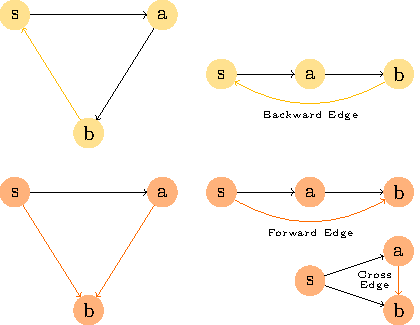
\includegraphics[width=0.5\textwidth, center]{./figures/dfs.pdf}
                  \end{minipage}
                }
                \resizebox{\textwidth}{!}{
                  \begin{minipage}[t]{11cm}
                    \dfs
                  \end{minipage}
                }
              }
              child {
                node {Recursive Depth-First Search
                  \resizebox{\textwidth}{!}{
                    \begin{minipage}[t]{11cm}
                      \dfsrec
                    \end{minipage}
                  }
                }
              }
              child {
                node {Depth-Limited Search}
                child {
                  node {Iterative-Deepening Search}
                }
              }
            }
          }
          % SEARCHEND
          % SEARCHSTART
          child {
            node {Informed Search Algorithms
              \resizebox{\textwidth}{!}{
                \begin{minipage}[t]{8cm}
                  \begin{itemize}
                    \item Knowledge of the worth of expanding a node $v$ is given in the form of an \alert{evaluation function} $f(v)$, which assigns a real number to each node
                    \item Often $f(v)$ includes a \alert{heuristic function} $h(v)$ as a component, which estimates the costs of the cheapest path from $v$ to the goal
                  \end{itemize}
                \end{minipage}
              }
            }
            child {
              node {Local Search Algorithms
                \resizebox{\textwidth}{!}{
                  \begin{minipage}[t]{8cm}
                    \begin{itemize}
                      \item if it is unimportant how the goal is reached, \alert{only the goal itself matters} and if in addition a \alert{quality} measure for nodes is given
                      \item it operates using a \alert{single current node} (rather than multiple paths)
                      \item requires little memory
                    \end{itemize}
                  \end{minipage}
                }
              }
              child {
                node {Hill Climbing
                  \resizebox{\textwidth}{!}{
                    \begin{minipage}[t]{8cm}
                      \begin{itemize}
                        \item Begin with a randomly-chosen configuration and \alert{improve} on it \alert{step by step}
                      \end{itemize}
                    \end{minipage}
                  }
                }
                child {
                  node {Simulated Annealing
                    \resizebox{\textwidth}{!}{
                      \begin{minipage}[t]{8cm}
                        \begin{itemize}
                          \item \enquote{noise} is injected systematically, first a lot, then gradually less
                        \end{itemize}
                      \end{minipage}
                    }
                  }
                }
                child {
                  node {Gradient Descent}
                }
              }
            }
            child {
              node {Genetic Algorithms
                \resizebox{\textwidth}{!}{
                  \begin{minipage}[t]{8cm}
                    \begin{itemize}
                      \item Similar to \alert{evolution}, we search for solutions by three operators: \alert{mutation}, \alert{crossover}, and \alert{selection}
                    \end{itemize}
                  \end{minipage}
                }
              }
            }
            child {
              node (bfs) {Best-First Search 
                \resizebox{\textwidth}{!}{
                  \begin{minipage}[t]{8cm}
                    \begin{itemize}
                      \item informed search procedure that expands the node with the \enquote{\alert{best}} $f$-value first
                      \item is an instance of the general \alert{Tree-Search} algorithm in which frontier is a \alert{priority queue} ordered by an \alert{evaluation function} $f$
                        \begin{itemize}
                          \item when $f$ is always correct, ones does not need to search
                        \end{itemize}
                    \end{itemize}
                  \end{minipage}
                }
              }
              child {
                node {Greedy Search
                  \resizebox{\textwidth}{!}{
                    \begin{minipage}[t]{8cm}
                      \begin{itemize}
                        \item A \alert{best-first} search using the \alert{heuristic function} $h(v)$ as the \alert{evaluation function}, i.e. $f(v) = h(v)$ is called a \alert{greedy search}
                          \begin{itemize}
                            % \item judge the \enquote{worth} of a node by estimating its path costs to the target node
                            \item $h(v) =$ estimated path-costs from $v$ to the target node
                            \item the only real restriction is that $h(v) = 0$ if $v$ is the target node
                          \end{itemize}
                        \item is generally \alert{incomplete} and \alert{not optimal}
                          \begin{itemize}
                            \item \alert{graph-search} version is complete only in finite graphs
                          \end{itemize}
                      \end{itemize}
                    \end{minipage}
                  }
                }
                child {
                  node (hf) {Heuristic function
                    \resizebox{\textwidth}{!}{
                      \begin{minipage}[t]{8cm}
                        \begin{itemize}
                          \item or simply a \alert{heuristic}
                          \item the evaluation function $f$ in \alert{greedy searches} is a heuristic function $h$ 
                          \item the heuristic is \alert{problem-specific} and \alert{focuses} the search
                          \item \alert{In AI it has two meanings:}
                            \begin{itemize}
                              \item Heuristics are \alert{fast} but in certain situations \alert{incomplete} methods for problem-solving
                              \item Heuristics are methods that \alert{improve the search} in the \alert{average-case}
                            \end{itemize}
                          \item The word heuristic is derived from the Greek word {\gyre ευρισκειν} (note also: {\gyre ευρηκα!})
                        \end{itemize}
                      \end{minipage}
                    }
                  }
                }
              }
              child {
                node (astar) {A$^*$
                  \resizebox{\textwidth}{!}{
                    \begin{minipage}[t]{8cm}
                      \begin{itemize}
                        \item A$^*$ combines \alert{greedy search} with the \alert{uniform-cost search}
                        \item Always expands node with lowest \alert{evaluation function} $f(v)$ first, where:
                          \begin{itemize}
                            \item $g(v) =$ actual cost from the start node to $v$
                            \item $h(v) =$ estimated cost from $v$ to the nearest target node
                            \item $f(v) = g(v) + h(v) =$ the estimated cost of the cheapest path through $v$
                          \end{itemize}
                        \item We require that for A$^*$, that $h$ is admissible (e.g. straight-line distance is admissible)
                          \begin{itemize}
                            \item $h$ is an \alert{optimistic estimate} of the costs that actually occur
                          \end{itemize}
                        \item \alert{complete}, provided that every node has a finite number of successor nodes and there exists a positive constant $\delta > 0$ such that every edge has at least weight $\delta$ and \alert{optimal}, provided that one uses the \alert{tree-based} variant
                          \begin{itemize}
                            \item for the \alert{graph-based} variant, one:
                              \begin{itemize}
                                \item either needs to consider re-opening nodes from the explored set, when a better estimate becomes known, or
                                \item one needs needs to require stronger restrictions on the heuristic estimate: it needs to be \alert{consistent}
                                \item $A^*$ can still be applied if heuristic is not consistent, but \alert{optimality is lost} in this case
                              \end{itemize}
                          \end{itemize}
                        \item \alert{Time complexity:} $O(b^d)$, exponential in the path length of the solution. More refined complexity results depend on the assumptions made, e.g. on the quality of the heuristic function
                        \item \alert{Space complexity:} $O(b^d)$, exponential in the path length of the solution. Roughly the same as that of all other graph search algorithms, as it keeps all generated nodes in memory
                      \end{itemize}
                    \end{minipage}
                  }
                }
                child {
                  node {Iterative-Deepening A$^*$ (IDA$^*$)
                    %     \resizebox{\textwidth}{!}{
                    %       \begin{minipage}[t]{8cm}
                    %         \begin{itemize}
                    %           \item the $f$-costs are used to define the cutoff (rather than the depth of the search tree)
                    %         \end{itemize}
                    %       \end{minipage}
                    %     }
                  }
                }
                child {
                  node {Recursive Best First Search (RBFS)}
                }
                child {
                  node {Memory-bounded A$^*$ (MA$^*$) and Simplified MA$^*$ (SMA$^*$)}
                }
                child {
                  node {Admissible
                    \resizebox{\textwidth}{!}{
                      \begin{minipage}[t]{8cm}
                        \begin{itemize}
                          \item $h$ is admissible if the following holds for all $v$: $h(v) \le h^*(v)$
                            \begin{itemize}
                              \item $h^*(v)$ are the actual cost of the optimal path from $v$ to the target node
                            \end{itemize}
                        \end{itemize}
                      \end{minipage}
                    }
                  }
                }
                child {
                  node {Consistent
                    \resizebox{\textwidth}{!}{
                      \begin{minipage}[t]{8cm}
                        \begin{itemize}
                          \item A heuristic $h$ is called consistent \alert{iff} for all edges $v$ leading from $s$ to $s'\colon h(s) - h(s') \le c(v)$, where $c(v)$ denotes the weight of edge $v$
                          \item Consistent heuristics prevent the need to re-open nodes from the explored set
                          \item Consistency implies \alert{admissibility}
                        \end{itemize}
                      \end{minipage}
                    }
                  }
                }
              }
            }
          } 
          % SEARCHEND
        }
        child {
          node {Trees
            \resizebox{\textwidth}{!}{
              \begin{minipage}[t]{12cm}
                \begin{itemize}
                  \item a graph with no cycle is \alert{acyclic}
                  \item a \alert{forest} is an acyclic graph
                  \item a \alert{tree} is a connected acyclic graph
                  \item a \alert{leaf} is a vertex of degree $1$
                  \item \underline{\href[page=59]{\lpathgraph{Graphentheorie_english_all_in_one_with_go_back.pdf}}{interesting properties}}
                    \begin{itemize}
                      \item every tree with at least two vertices has at least two leaves
                      \item deleting a leaf from an $n$-vertex tree produces a tree with $n-1$ vertices
                      \item for an $n$-vertex simple graph $G$ (with $n\ge 1$) the following are equivalent:
                        \begin{enumerate}
                          \item $G$ is connected and has no cycles
                          \item $G$ is connected and has $n-1$ edges
                          \item $G$ has $n-1$ edges and no cycles
                          \item for $u, v \in V(G)$, $G$ has exactly one $u, v$-path
                        \end{enumerate}
                      \item every edge of a tree is a cut-edge
                      \item adding one edge to a tree forms exactly one cycle
                    \end{itemize}
                \end{itemize}
              \end{minipage}
            }
          }
          child {
            node {Directed Trees
              \resizebox{\textwidth}{!}{
                \begin{minipage}[t]{12cm}
                  \begin{itemize}
                    \item a \alert{rooted tree (germ. gewurzelter Baum)} $T$ is a simple digraph with a vertex $r$ chosen as root such that for each vertex $v\in V(T)$ there's a unique path \alert{$P(v)$}  from $r$ to $v$
                    \item the \alert{parent} of $v\ne r$ is the predecessor in $P(v)$
                    \item the \alert{children} of $v$ are the \alert{sucessor set} $N^+(v)$ of $v$
                    \item the \alert{ancestors} of $v$ are all vertices of $P(v) - v$
                    \item the \alert{descendants} of $v$ are all vertices $u\ne v$ such that $P(u)$ contains the vertex $v$
                    \item the \alert{leaves} are vertices with no children
                    \item a \alert{rooted plane tree} or \alert{planted tree (germ. gewurzelter Baum mit Kantenorientierung/Kantenbeschriftung)} is a rooted tree with a given (left/right) ordering or labeling specified for all children of each vertex
                  \end{itemize}
                  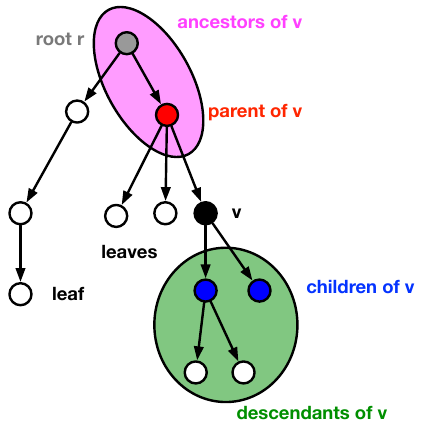
\includegraphics[width=0.6\textwidth, center]{./figures/directed_tree.png}
                \end{minipage}
              }
            }
            child {
              node {Binary Tree
                \resizebox{\textwidth}{!}{
                  \begin{minipage}[t]{12cm}
                    \begin{itemize}
                      \item a \alert{binary tree} is
                        \begin{itemize}
                          \item a rooted plane tree
                          \item where each vertex has at most two children
                          \item and each child of a vertex is designated as its
                            \begin{itemize}
                              \item \alert{left child} or
                              \item \alert{right child}
                            \end{itemize}
                        \end{itemize}
                      \item the subtrees rooted at the root are
                        \begin{itemize}
                          \item the \alert{left subtree} and
                          \item the \alert{right subtree}
                        \end{itemize}
                      \item a \alert{$k$-ary tree} allows each vertex up to $k$ children
                    \end{itemize}
                    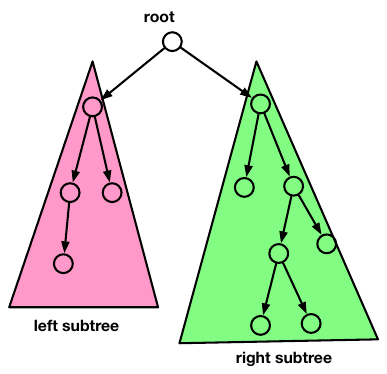
\includegraphics[width=0.6\textwidth, center]{./figures/binary_tree.png}
                  \end{minipage}
                }
              }
            }
            child {
              node {Dominator Tree
                \resizebox{\textwidth}{!}{
                  \begin{minipage}[t]{12cm}
                    \begin{itemize}
                      \item rooted tree described by the root vertex $r$ and the edges described by $u \operatorname{idom} v$
                      \item for a flowgraph $G=(V,E,r)$ a vertex $v$ \alert{dominates} a vertex $w \ne v$: ($v \operatorname{dom} w$) if every path in $G$ from $r$ to $w$ contains $v$
                      \item for a flowgraph $G=(V,E,r)$ a vertex $v$ is an \alert{immediate dominator} of $w$: ($v \operatorname{idom} w$) if ($v \operatorname{dom} w$) and there is no vertex $u$ such that ($v \operatorname{dom} u$) and ($u \operatorname{dom} w$)
                      \item \href[page=93]{\lpathgraph{Graphentheorie_english_all_in_one_with_go_back.pdf}}{Lemma}:
                        \begin{itemize}
                          \item $(u \operatorname{dom} v) \operatorname{and} (v \operatorname{dom} w) \Rightarrow (u \operatorname{dom} w)$
                          \item $(u \operatorname{dom} w) \operatorname{and} (v \operatorname{dom} w) \Rightarrow (u \operatorname{dom} v) \operatorname{or} (v \operatorname{dom} u)$
                          \item $(u \operatorname{dom} v) \Rightarrow \neg (v \operatorname{dom} u)$
                          \item $\forall v \ne r: \exists! u: (u \operatorname{idom} v)$
                        \end{itemize}
                      \item \href[page=96]{\lpathgraph{Graphentheorie_english_all_in_one_with_go_back.pdf}}{algorithm}
                    \end{itemize}
                  \end{minipage}
                }
              }
              child {
                node {Flowgraph
                  \resizebox{\textwidth}{!}{
                    \begin{minipage}[t]{12cm}
                      \begin{itemize}
                        \item a \alert{flowgraph} $G=(V,E,r)$ is 
                          \begin{itemize}
                            \item a digraph $(V, E)$
                            \item with start vertex $r$
                            \item such that for any vertex $v \in V$
                            \item there is a path from $r$ to $v$
                          \end{itemize}
                        \item a \alert{program flowgraph} is
                          \begin{itemize}
                            \item a flowgraph with maximum outdegree $2$
                          \end{itemize}
                      \end{itemize}
                    \end{minipage}
                  }
                }
              }
              child {
                node {Control Flow Graphs (CFG's) (germ. Kontrollflussgraphen)
                  \resizebox{\textwidth}{!}{
                    \begin{minipage}[t]{12cm}
                      \begin{itemize}
                        \item \alert{Control Flow Graph (CFG):}
                          \begin{itemize}
                            \item Given a program code $P$
                            \item each reachable line represents a vertex in the flowgraph
                            \item the first executed line is $r$ of the flowgraph
                            \item edge $(u,v)$ is in the flowgraph
                              \begin{itemize}
                                \item if and only if the control can jump from line $u$ to line $v$
                              \end{itemize}
                            \item alia for determining \alert{dominators}, i.e. Code lines guaranteed to be executed before other code
                          \end{itemize}
                        \item \alert{well structured / reducible CFG:} edges are either forward edges or back edges
                          \begin{itemize}
                            \item \alert{forward edges} form an acyclic graph reached from the entry node
                            \item \alert{back edges} consist only of edges whose targets dominate their sources
                          \end{itemize}
                      \end{itemize}
                    \end{minipage}
                  }
                }
              }
            }
            child {
              node {Code Tree
                \resizebox{\textwidth}{!}{
                  \begin{minipage}[t]{12cm}
                    \begin{itemize}
                      \item \href[page=83]{\lpathgraph{Graphentheorie_english_all_in_one_with_go_back.pdf}}{definition}
                      \item example \href[page=84]{\lpathgraph{Graphentheorie_english_all_in_one_with_go_back.pdf}}{Huffman Coding}
                    \end{itemize}
                  \end{minipage}
                }
              }
            }
          }
          child {
            node {Spanning Trees (germ. Spannbäume)
              \resizebox{\textwidth}{!}{
                \begin{minipage}[t]{12cm}
                  \begin{itemize}
                    \item a \alert{spanning subgraph (germ. spannender Teilgraph)} of $G$ is a connected subgraph with vertex set $V(G)$
                    \item a \alert{spanning tree (germ. Spannbaum)} is a spanning subgraph of a given graph $G$ that is a tree
                    \item \underline{\href[page=69]{\lpathgraph{Graphentheorie_english_all_in_one_with_go_back.pdf}}{interesting properties}:}
                      \begin{itemize}
                        \item every connected graph contains a spanning tree
                        \item if $T, T'$ are spanning trees of a connected graph $G$ and $e\in E(T) - E(T')$ then there is a edge $e'\in E(T') - E(T)$ such that $T-e+e'$ is a spanning tree of $G$
                      \end{itemize}
                  \end{itemize}
                \end{minipage}
              }
            }
            child {
              node {Minimum Spanning Trees
                \resizebox{\textwidth}{!}{
                  \begin{minipage}[t]{12cm}
                    \begin{itemize}
                      \item a \alert{spanning tree} whose sum of \alert{edge weights} is as \alert{small as possible}
                      \item for minimum spanning trees we consider only \alert{non-negative edge weights}
                        % \item \alert{weighted graph}: a graph with numerical labels on the edges, so-called edge weights
                    \end{itemize}
                  \end{minipage}
                }
              }
            }
            child {
              node {Kruskal’s Algorithm
                \resizebox{\textwidth}{!}{
                  \begin{minipage}[t]{12cm}
                    \begin{itemize}
                      \item in a connected weighted graph $G$ Kruskal’s algorithm constructs a minimum-weight spanning tree
                      \item \href[page=75]{\lpathgraph{Graphentheorie_english_all_in_one_with_go_back.pdf}}{algorithm}
                    \end{itemize}
                  \end{minipage}
                }
              }
            }
          }
          child {
            node {Distance, Diameter, Eccentricity, Radius and Center
              \resizebox{\textwidth}{!}{
                \begin{minipage}[t]{12cm}
                  \begin{itemize}
                    \item \alert{distance} $d_G(u, v)$: the least (shortest) length of a $u, v$-path (if $G$ has a $u, v$-path)
                      \begin{itemize}
                        \item if $G$ has no such path then $d_G(u, v) = \infty$
                      \end{itemize}
                    \item \alert{diameter}: $diam(G) := max_{u, v\in V(G)} d(u, v)$
                      \begin{itemize}
                        \item for a simple graph $G$: $diam(G)\ge 3 \Rightarrow diam(\overline{G}) \le 3$
                      \end{itemize}
                    \item \alert{eccentricity}: $\epsilon(u) := max_{v\in V(G)} d(u, v)$
                      % \item \alert{radius}: $rad(G) := min_{u\in V(G)} \epsilon(u, v)$
                    \item \alert{radius}: $rad(G) := min_{u\in V(G)} \epsilon(u)$
                    \item the \alert{center} of a graph $G$ is the subgraph induced by the vertices of minimum eccentricity
                      \begin{itemize}
                        \item the \alert{center of a tree} is a vertex or an edge
                      \end{itemize}
                  \end{itemize}
                \end{minipage}
              }
            }
          }
        }
      child {
        node {Dual Problems
          \resizebox{\textwidth}{!}{
            \begin{minipage}[t]{12cm}
              \begin{itemize}
                \item \alert{Min-max relation:} States
                  \begin{itemize}
                    \item the equality of the solution of a minimization problem and a maximization problem
                    \item the optimality of both solutions
                  \end{itemize}
              \end{itemize}
            \end{minipage}
          }
        }
        child {
          node {$x,y$-edge-cut and pairwise edge-disjoint $x,y$-paths
            \resizebox{\textwidth}{!}{
              \begin{minipage}[t]{12cm}
                \begin{itemize}
                  \item $\kappa'_D(x, y) \ge \lambda'_D(x, y)$
                  \item \alert{Menger’s Theorem:} If $x\ne y$ then $\lambda'(x, y) = \kappa'(x, y)$
                \end{itemize}
              \end{minipage}
            }
          }
          child {
            node (edgecut)  {$x,y$-edge-cut or $x,y$ edge-separator
              \resizebox{\textwidth}{!}{
                \begin{minipage}[t]{12cm}
                  \begin{itemize}
                    \item a set $E' \subseteq E$ is an \alert{$x,y$ edge-separator} or \alert{$x,y$-edge-cut} if $G - E'$ has no $x,y$-path
                    \begin{itemize}
                      \item $\kappa'(x, y)$ is the minimum number of edges whose deletion make $y$ unreachable from $x$
                    \end{itemize}
                  \end{itemize}
                \end{minipage}
              }
            }
          }
          child {
            node {Pairwise edge-disjoint $x,y$-paths
              \resizebox{\textwidth}{!}{
                \begin{minipage}[t]{12cm}
                  \begin{itemize}
                    \item $\lambda'(x, y)$ is the maximum size of a set of \alert{pairwise edge-disjoint $x,y$-paths}
                  \end{itemize}
                \end{minipage}
              }
            }
          }
        }
        child {
          node {Coloring and Cliques
            \resizebox{\textwidth}{!}{
              \begin{minipage}[t]{8cm}
                \begin{itemize}
                  \item \alert{Chromatic number $\chi(G)$}: Is the \alert{minimum} number of colors such that \alert{adjacent vertices} receive \alert{different colors}
                  \item for every graph $G$: $\chi(G)\ge \omega(G)$
                \end{itemize}
              \end{minipage}
            }
          }
          child {
            node (coloring) {Coloring
              \resizebox{\textwidth}{!}{
                \begin{minipage}[t]{12cm}
                  \begin{itemize}
                    \item \alert{k-coloring} of a graph is a labeling $f : V(G) \rightarrow S$ where $|S| = k$
                      \begin{itemize}
                        \item the labels are \alert{colors}
                      \end{itemize}
                    \item vertices of one color form a \alert{color class}
                      \begin{itemize}
                        \item each color class is an \alert{independent set}
                      \end{itemize}
                    \item a graph is \alert{$k$-colorable} if it has a proper $k$-coloring
                      \begin{itemize}
                        \item a $k$-coloring is \alert{proper} if adjacent vertices have different labels
                        \item $k$-colorable and \alert{$k$-partite} have the same meaning
                        \item graphs with \alert{loops} are \alert{uncolorable}
                        \item \alert{multiple edges} are \alert{irrelevant}
                        \item \href[page=212]{\lpathgraph{Graphentheorie_english_all_in_one_with_go_back.pdf}}{Test for $2$-colorability}
                        \item \alert{Chromatic number $X(G)$:} is the least $k$ such that $G$ is $k$-colorable
                          \begin{itemize}
                            \item a graph is \alert{$k$-chromatic} if $\chi(G) = k$
                            \item a proper $k$-coloring of a $k$-chromatic graph is an \alert{optimal coloring}
                            \item every $k$-chromatic graph with n vertices has at least $\displaystyle \binom{k}{2} = \sum^{k-1}_{i=0} i$ edges. Equality holds for a complete graph plus isolated vertices
                            \item for \alert{disjoint union:} $\chi(G+H) = max\{\chi(G), \chi(H)\}$
                            \item for \alert{join:} $\chi(G\vee H) = \chi(G) + \chi(H)$
                            \item for \alert{cartesian:} $\chi(G\square H) = max\{\chi(G), \chi(H)\}$
                          \end{itemize}
                      \end{itemize}
                    \item if $\chi(H) < \chi(G) = k$ for every proper subgraph $H$ of $G$, then $G$ is \alert{color-critical} or \alert{$k$-critical}
                      \begin{itemize}
                        \item properly coloring a graph needs at least $2$ colors \alert{iff} the graph has an edge
                        \item $K_2$ is the only $2$-critical graph
                        \item since $2$-colorable is the same as bipartite characterization of bipartite graphs implies: $3$-critical graphs are the odd cycles
                        \item every $k$-critical graph is $k-1$-edge-connected
                      \end{itemize}
                    \item \href[page=222]{/home/areo/Documents/Studium/Summaries/Graph_Theory/Graphentheorie_all_in_one_with_go_back.pdf}{greedy coloring algorithm} and \href[page=223]{/home/areo/Documents/Studium/Summaries/Graph_Theory/Graphentheorie_all_in_one_with_go_back.pdf}{improvements}
                    \item \alert{upper bound:} $\chi(G)\le \Delta(G) + 1$
                    \item \alert{Lemma (Kainen):} Let $G$ be a graph with $\chi(G) > k$. Let $X$, $Y$ be a partition of $V(G)$. If $G[X]$ and $G[Y]$ are $k$-colorable \alert{then} the edge cut $[X,Y]$ has at least $k$ edges
                  \end{itemize}
                \end{minipage}
              }
            }
          }
          child {
            node (clique) {Clique
              \resizebox{\textwidth}{!}{
                \begin{minipage}[t]{12cm}
                  \begin{itemize}
                    \item is a set of \alert{pairwise adjacent vertices}
                      \begin{itemize}
                        \item \alert{Clique number (germ. Cliquenzahl) $\omega(G)$:} Size (number of vertices) of the largest clique
                      \end{itemize}
                  \end{itemize}
                \end{minipage}
              }
            }
          }
        }
        child {
          node {Minimum-Cut and Maximum-Flow
            \resizebox{\textwidth}{!}{
              \begin{minipage}[t]{12cm}
                \begin{itemize}
                  \item a \alert{network} is a \alert{digraph} $G = (V, E)$ with \alert{capacity} $c(e)\ge 0$ on each edge $e\in E$, a \alert{source vertex} $s\in V$ and a \alert{sink vertex} $t\in V$
                  \item \alert{weak duality:} If $f$ is a \alert{feasible flow} and $[S,T]$ is a \alert{source/sink cut} then $val(f) = f^+(S) - f^-(S) \le f^+(S) \le cap(S, T)$
                    \begin{itemize}
                      \item the total flow on edges \alert{leaving} $U$ is $\displaystyle f^{+}(U)=\sum_{\mathclap{\substack{u \in U, v \in V \backslash U, u v \in E}}} f(u v)$
                      \item the total flow on edges \alert{entering} $U$ is $\displaystyle f^{-}(U)=\sum_{\mathclap{\substack{v \in V\backslash U, u \in U , v u \in E}}} f(v u)$
                      \item the \alert{net flow} of $U$ is $f^+(U) − f^−(U)$
                      \item if $U$ is a set of nodes in a network then the net flow out of $U$ is the sum of net flows out of the nodes in $U$, i.e. $\displaystyle f^+(U) − f^−(U) = \sum_{v\in U} (f^+(v) − f^−(v))$
                      \item in particular if $f$ is a feasible flow and $[S,T]$ is a source/sink cut then the net flow out of $S$ and net flow into $T$ equal $val(f)$
                    \end{itemize}
                  \item \alert{Max-Flow Min-Cut Theorem:}  $\displaystyle \max_{f} val(f) = \min_{S, T} cap(S, T)$, in every network, the maximum value of a feasible flow equals the minimum capacity of a source/sink cut
                    \begin{itemize}
                      \item Max flow and Min cut problems on a network are a dual optimization problem. Given a flow with value $\alpha$ and a cut with capacity $\alpha$, the weak duality above proves that the cut is minimum cut and the flow is maximum flow. If every instance has solutions with the same value to both the max problem and the min problem (\enquote{strong duality}), then a short proof of optimality always exists
                      \item the \href[page=201]{\lpathgraph{Graph_Theory/Graphentheorie_all_in_one_with_go_back.pdf}}{proof} requires rational capacities otherwise the algorithm may yield augmenting path forever
                    \end{itemize}
                \end{itemize}
              \end{minipage}
            }
          }
          child {
            node (cut) {Cut
              \resizebox{\textwidth}{!}{
                \begin{minipage}[t]{12cm}
                  \begin{itemize}
                    \item a \alert{source/sink cut $[S, T]$} consists of the \alert{edges} from a \alert{source set $S$} to a \alert{sink set $T$}
                      \begin{itemize}
                        \item partition $S$, $T$ with $s \in S$, $t \in T$ of the node set $V$ of a network $G=(V,E)$
                      \end{itemize}
                    \item the \alert{capacity} of the cut $[S, T]$ is $\displaystyle cap(S, T) = \sum_{\mathclap{\substack{u\in S, v\in T}}} c(uv)$
                      \begin{itemize}
                        \item edges from $T$ to $S$ do not affect the capacity of the cut
                      \end{itemize}
                    \item \alert{Minimum Cut Problem}: Given a network problem find a minimum cut $(S,T)$ which minimizes $cap(S,T)$
                  \end{itemize}
                \end{minipage}
              }
            }
          }
          child {
            node {Flow
              \resizebox{\textwidth}{!}{
                \begin{minipage}[t]{12cm}
                  \begin{itemize}
                    \item a \alert{flow $f$} assigns a \alert{value $f(e)$} to each edge $e$ 
                    \item $\displaystyle f^+(v) = \sum_{vw\in E} f(vw)$ is the flow \alert{leaving} vertex $v$ 
                    \item $\displaystyle f^−(v) = \sum_{wv\in E} f(wv)$ is the flow \alert{entering} a vertex $v$ 
                    \item the \alert{net flow} of $v$ is $f^−(v) − f^+(v)$
                    \item a flow $f$ is \alert{feasible} if it satisfies the \alert{capacity constraints} $\forall e\in E:0\leq f(e)\leq c(e)$ and the \alert{conservation constraints} $\forall\nu\in V\setminus\{s,t\}:f^{+}(\nu)=f^{-}(\nu)$
                    \item \alert{flow value} $val(f) = f^-(t) - f^+(t) = f^+(s) - f^-(s)$ is the network flow into the sink
                    \item \alert{Max-Flow-Problem:} For a network find a feasible flow $f$ with maximum flow value
                      % \item flow \alert{from} the node $v$: $\displaystyle f^+(v) = \sum_{vw\in E} f((v,w))$ 
                      % \item flow \alert{into} the node $v$: $\displaystyle f^-(v) = \sum_{wv\in E} f((w,v))$
                  \end{itemize}
                \end{minipage}
              }
            }
            child {
              node {Integral Flow
                \resizebox{\textwidth}{!}{
                  \begin{minipage}[t]{12cm}
                    \begin{itemize}
                      \item An \alert{integral flow} is a flow using only integer capacites
                      \item \alert{Integrality Theorem:} If all capacities in a network are integers, then there is a maximum flow assigning integral flow to each edge
                        \begin{itemize}
                          \item Furthermore, some maximum flow can be partitioned into flows of unit value along paths from source to sink
                        \end{itemize}
                    \end{itemize}
                  \end{minipage}
                }
              }
            }
          }
          child {
            node {Ford-Fulkerson Labeling Algorithm
              \resizebox{\textwidth}{!}{
                \begin{minipage}[t]{12cm}
                  \begin{itemize}
                    \item \href[page=193]{\lpathgraph{Graphentheorie_all_in_one_with_go_back.pdf}}{algorithm with example}
                      \begin{itemize}
                        \item modifications by \href[page=204]{\lpathgraph{Graphentheorie_all_in_one_with_go_back.pdf}}{Edmonds und Karp}
                      \end{itemize}
                    \item \alert{f-augmenting path $P$} is a source-to-sink path $P$ in the underlying graph $G$ such that for each $e\in E(P)$: 
                      \begin{itemize}
                        % \item  paths are considered in the undirected version of the network $N$
                        \item $P$ follows $e$ forward, then $f(e) < c(e)$
                        \item $P$ follows $e$ backward, then $f(e) > 0$
                      \end{itemize}
                    \item \alert{tolerance} of $\displaystyle\epsilon(P) = \min_{e\in E(P)} \epsilon(e)$
                      \begin{itemize}
                        \item $\epsilon(e) = c(e) - f(e)$ if $e$ is \alert{forward} in $P$
                        \item $\epsilon(e) = f(e)$ if $e$ is \alert{backward} in $P$
                      \end{itemize}
                    \item an $f$-augmenting path leads to a flow with larger value, \alert{Lemma:}
                      \begin{itemize}
                        \item If $P$ is an $f$-augmenting path with tolerance $z$
                          \begin{itemize}
                            \item then change flow by $+z$ on forward edges of $P$
                            \item and change flow by $-z$ on backward edges of $P$
                          \end{itemize}
                        \item produces a feasible flow $f’$ with $val(f’)= val(f) + z$
                      \end{itemize}
                    \item \alert{Remarks:}
                      \begin{itemize}
                        \item adding a path does not always lead to the maximum flow
                        \item flow on backward edges does not disappear, it is redirected
                        \item augmentation cuts the flow and extends each portion to become a new flow path
                        \item a flow is a maximal flow if there is a \enquote{bottleneck} described by the capacity from $s$ to $t$
                      \end{itemize}
                  \end{itemize}
                \end{minipage}
              }
            }
          }
        }
        child {
          node {Weighted Matching and Weighted Vertex Cover
            \resizebox{\textwidth}{!}{
              \begin{minipage}[t]{12cm}
                \begin{itemize}
                  % \item \alert{equality subgraph (germ. Gleichheitsteilgraph) $G_{u,v}$} for a weighted cover $(u,v)$ is the spanning subgraph of $K_{n,n}$ having the edges $x_iy_j$ such that $u_i + v_j = w_{i,j}$
                  \item $G_{u,v}$ has a \alert{perfect matching $M$} if the weight $\displaystyle\sum_{u_iv_j\in M} w_{i,j}$ is equal to $\displaystyle\sum_i u_i + \sum_j v_j$
                    \begin{itemize}
                      \item \underline{we then have a optimal solution because of the following lemma:}
                      \begin{itemize}
                        \item for a \alert{perfect matching $M$} and \alert{weighted cover $(u,v)$} in a weighted bipartite graph $G$ it applies that: $c(u,v) \ge w(M)$
                        \item $c(u,v) = w(M)$ \alert{iff} $M$ consists of edges $ij$ such that $u_i + v_j = w_{i,j}$
                      \end{itemize}
                    \end{itemize}
                    % \begin{itemize}
                    %   \item and by the Lemma above that is a optimal solution
                    %   \item otherwise we find a matching $M$ and a vertex cover $Q$ of the same size
                    % \end{itemize} makes no sense
                    % \item if $G_{u,v}$ has a \alert{perfect matching} then its weight is $\displaystyle\sum_i u_i + \sum_j v_j$
                    %   \begin{itemize}
                    %     \item and by Lemma 3.2.7 we have the optimal solution
                    %     \item otherwise we find a matching $M$ and a vertex cover $Q$ of the same size
                    %   \end{itemize}
                    % \item if $G_{u,v}$ has a \alert{perfect matching} then its weight $\displaystyle\sum_{u_{i},v_{j}in M}w_{i,j}$ is equal to $\displaystyle\sum_{i}u_{i}+{{\sum_{j}}}\;\nu_{j}$
                \end{itemize}
              \end{minipage}
            }
          }
          child {
            node {Maximum Weighted Matching Problem / Assignment Problem
              \resizebox{\textwidth}{!}{
                \begin{minipage}[t]{12cm}
                  \begin{itemize}
                    % \item find a transversal $M$ (perfect matching $M$ in $K_{n,n}$) with maximum sum $\displaystyle w(M) = \sum_{ij\in M} w_{ij}$
                    \item find a transversal $M$ (perfect matching) with maximum sum $\displaystyle w(M) = \sum_{ij\in M} w_{ij}$
                    \begin{itemize}
                      \item a \alert{transversal} $M$ of an $n \times n$ matrix consists of $n$ positions, one in each row and each column
                    \end{itemize}
                  \end{itemize}
                \end{minipage}
              }
            }
          }
          child {
            node {Minimum Weighted Vertex Cover Problem
              \resizebox{\textwidth}{!}{
                \begin{minipage}[t]{12cm}
                  \begin{itemize}
                      % \item for $u = (u_1, \ldots u_n)$, $v = (v_1, \ldots, v_n)$ is (weighted) \alert{$(u,v)$-Cover} of $w$, if $u_i + v_j \ge w_{i,j}$ for all $i$, $j$
                    \item find a weighted cover $(u,v)$ of minimum cost
                      \begin{itemize}
                        \item \alert{(weighted) $(u,v)$-Cover} is a choice of labels $u = (u_1, \ldots, u_n)$, $v = (v_1, \ldots, v_n)$ such that $u_i + v_j \ge w_{i,j}$ for all $i$, $j$
                        \item \alert{cost} of a cover $(u,v)$ is $\displaystyle c(u,v) = \sum_i u_i + \sum_j v_j$
                      \end{itemize}
                  \end{itemize}
                \end{minipage}
              }
            }
          }
          child {
            node {Hungarian Algorithm
              \resizebox{\textwidth}{!}{
                \begin{minipage}[t]{12cm}
                  \begin{itemize}
                    \item \href[page=163]{\lpathgraph{Graphentheorie_all_in_one_with_go_back.pdf}}{algorithm with example} and \href[page=122]{\lpathgraph{Graphentheorie_exercise_class_slides_all_in_one_with_go_back.pdf}}{another example}
                      % \item the \alert{Hungarian Algorithm} finds a \alert{maximum weight matching} and a \alert{minimum cost cover}
                    \item the \alert{Hungarian Algorithm} finds a \alert{maximum weighted matching} and a \alert{minimum weighted vertex cover}
                    \item \alert{equality subgraph (germ. Gleichheitsteilgraph) $G_{u,v}$} for a weighted cover $(u,v)$ is the spanning subgraph of $K_{n,n}$ having the edges $ij$ such that $u_i + v_j = w_{i,j}$
                    \item for the weighted cover $u_1, \ldots, u_n$, $v_1, \ldots, v_n$ and weights $w_{i, j} \ge 0$ the \alert{excess matrix} is $c_{i,j} = u_{i}+ v_{j} - w_{i,j}$
                    % \item stop \enquote{production:} $u_{i}+v_{j}>w_{i,j}$ and at the same time minimize $\sum_{i}u_{i}+\sum_{j}\nu_{j}$
                  \end{itemize}
                \end{minipage}
              }
            }
          }
        }
        child {
          node {Matching and Vertex cover
            \resizebox{\textwidth}{!}{
              \begin{minipage}[t]{8cm}
                \begin{itemize}
                  \item the size of a \alert{vertex cover} is always \alert{at least as big as} the size of a \alert{matching} (Size of vertex cover $\ge$ Size of matching)
                    \begin{itemize}
                      \item each edge of a matching has at least one covering vertex
                      \item no vertex can cover two edges of a matching because edges are not incident in matchings
                        % \item no vertex can cover two edges of a matching edge because matched edges are not adjacent
                        % Jede Kante eines Matchings hat mindestens einen überdeckenden
                        % Knoten
                        % • Kein Knoten kann zwei Kanten eines Matchings abdecken
                        % • weil Kanten in Matchings nicht inzidieren
                    \end{itemize}
                  \item \alert{Theorem of König and Egerváry:} For any bipartite graph $G$ the size of maximum matching equals the size of minimum vertex cover
                \end{itemize}
              \end{minipage}
            }
          }
          child {
            node {Matching
              \resizebox{\textwidth}{!}{
                \begin{minipage}[t]{10cm}
                  \begin{itemize}
                    \item a \alert{matching $M$} in a graph $G$ is a set of non-loop edges with no shared endpoints
                      \begin{itemize}
                        \item the vertices incident to the edges of a matching M are \alert{$M$-saturated}
                        \item the other vertices are \alert{$M$-unsaturated}
                        \item a \alert{perfect matching} saturates every vertex
                        \item \underline{perfect matching in complete graphs:}
                          \begin{itemize}
                            \item \underline{even number of vertices:} $K_{2n+1}$ has no perfect matching because the number of vertices is odd
                            \item \underline{odd number of vertices:} $K_{2n}$ has  $f_n = (2n-1) \cdot f_{n-1} = (2n-1) \cdot \ldots \cdot 5 \cdot 3 \cdot 1$ perfect matchings for $n = \dfrac{|V(G)|}{2}$ (because the edges are undirected, there are $2n-1$ choices for the first pairing of a given node, as there are $2n$ nodes, but a node can't pair with himself, so $2n-1$)
                          \end{itemize}
                        \item the \alert{size} of a matching is given by the \alert{number of edges}
                        \item a \alert{maximal matching (germ. nicht erweiterbares)} in a graph is a matching that cannot be enlarged by adding an edge
                        \item a \alert{maximum matching (germ. größtmögliches / maximales)} is a matching of maximum size (among all matchings in a graph)
                        \item \alert{$\alpha'(G)$:} Is the maximum size of matching of edges in $G$
                      \end{itemize}
                  \end{itemize}
                \end{minipage}
              }
            }
            child {
              node (mec) {Other Connections
                \resizebox{\textwidth}{!}{
                  \begin{minipage}[t]{8cm}
                    \begin{itemize}
                      \item \alert{Theorem (Gallai):} If G is a graph without isolated vertices (without edges), then $\alpha'(G) + \beta'(G) = n(G)$
                    \end{itemize}
                  \end{minipage}
                }
              }
            }
            child {
              node {Theorem (Berge)
                \resizebox{\textwidth}{!}{
                  \begin{minipage}[t]{8cm}
                    \begin{itemize}
                      \item a matching $M$ in a graph $G$ is a maximum matching in $G$ \alert{iff} $G$ has no $M$-augmenting path
                    \end{itemize}
                  \end{minipage}
                }
              }
              child {
                node (apa) {Augmenting Path Algorithm
                  \resizebox{\textwidth}{!}{
                    \begin{minipage}[t]{8cm}
                      \begin{itemize}
                        \item \href[page=140]{\lpathgraph{Graphentheorie_english_all_in_one_with_go_back.pdf}}{algorithm}
                        \item \underline{Theorem:} Repeatedly applying the Augmenting Path Algorithm to a bipartite graph produces a \alert{matching} and a \alert{vertex cover} of equal size
                      \end{itemize}
                    \end{minipage}
                  }
                }
              }
              child {
                node {Alternating and Augmenting Paths
                  \resizebox{\textwidth}{!}{
                    \begin{minipage}[t]{8cm}
                      \begin{itemize}
                        \item given a matching $M$ in $G$, an \alert{$M$-alternating path} is a path that alternates between edges in $M$ and edges not in $M$ ($E(G)-M$)
                        \item an $M$-alternating path whose endpoints are unsaturated by $M$ is an \alert{$M$-augmenting path}
                      \end{itemize}
                    \end{minipage}
                  }
                }
              }
            }
            child {
              node {Theorem (Hall)
                \resizebox{\textwidth}{!}{
                  \begin{minipage}[t]{8cm}
                    \begin{itemize}
                      \item an $X$, $Y$-bigraph has a matching that saturates $X$ \alert{iff} $|N(S)| \ge |S|$ for all $S \subseteq X$
                    \end{itemize}
                  \end{minipage}
                }
              }
              % child {
              %   node {X,Y-Bigraph
              %     \resizebox{\textwidth}{!}{
              %       \begin{minipage}[t]{8cm}
              %         \begin{itemize}
              %           \item a bipartite graph with vertex sets $X$ and $Y$ and edges only between $X$ and $Y$
              %         \end{itemize}
              %       \end{minipage}
              %     }
              %   }
              % }
            }
            child {
              node {Complete Graphs
                \resizebox{\textwidth}{!}{
                  \begin{minipage}[t]{8cm}
                    \begin{itemize}
                      \item $K_{2n}$ has $f_n = (2n-1)\cdot f_{n-1} = 1\cdot 3\cdot 5\cdot (2n-1)$ choices for choices for perfect matchings
                        \begin{itemize}
                          \item $K_n$ is a complete graph with $n$ vertices, i.e. a simple graph with maximum number of edges
                        \end{itemize}
                      \item $K_{2n+1}$ has no perfect matching because the node number of vertices is odd
                    \end{itemize}
                  \end{minipage}
                }
              }
            }
            child {
              node {Regular bipartite graphs
                \resizebox{\textwidth}{!}{
                  \begin{minipage}[t]{8cm}
                    \begin{itemize}
                      \item for $k > 0$, every $k$-regular bipartite graph has a perfect matching
                    \end{itemize}
                  \end{minipage}
                }
              }
            }
            child {
              node (symmetricdifferencematching) {Symmetric Differences of Matchings
                \resizebox{\textwidth}{!}{
                  \begin{minipage}[t]{12cm}
                    \begin{itemize}
                      \item every component of the symmetric difference of two matchings of $G$ is
                        \begin{itemize}
                          \item a path or
                          \item an even cycle
                        \end{itemize}
                    \end{itemize}
                  \end{minipage}
                }
              }
            }
          }
          child {
            node (vc) {Vertex cover (germ. Knotenüberdeckung)
              \resizebox{\textwidth}{!}{
                \begin{minipage}[t]{10cm}
                  \begin{itemize}
                    \item a set $Q \subseteq V(G)$ that contains at least one endpoint of every edge
                      \begin{itemize}
                        \item the vertices $Q$ \enquote{cover} (germ. \enquote{überdecken}) $E(G)$
                        \item \alert{Minimum Vertex Cover (germ. Minimale Knotenüberdeckung) $\beta(G)$:} Is the minimum size of vertex cover of vertices in $G$ % Minimize the number of vertices $Q$ of a cover of $E(G)$
                      \end{itemize}
                    \item \href[page=129]{\lpathgraph{Graphentheorie_english_all_in_one_with_go_back.pdf}}{examples}
                  \end{itemize}
                \end{minipage}
              }
            }
          }
        }
        child {
          node {Independant Set and Edge cover
            \resizebox{\textwidth}{!}{
              \begin{minipage}[t]{8cm}
                \begin{itemize}
                  \item the size of a (minimal) edge cover is at least the size of a maximal independed set
                    \begin{itemize}
                      \item because no edge can cover more than one vertex of such a set\cite{ravskyAnswerRelationIndependent2017}
                    \end{itemize}
                \end{itemize}
              \end{minipage}
            }
          }
          child {
            node (independant set) {Independant Set (germ. Unabhängige Menge)
              \resizebox{\textwidth}{!}{
                \begin{minipage}[t]{8cm}
                  \begin{itemize}
                    \item vertices are \alert{independent}, if they are not connected via an edge
                    \item a set of pairwise nonadjacent vertices
                      \begin{itemize}
                        \item \alert{Independence number (germ. Unabhängigkeitszahl) $\alpha(G)$:} Is the maximum size of independent set of vertices in $G$
                      \end{itemize} 
                  \end{itemize}
                \end{minipage}
              }
            }
            child {
              node (isvccqcl) {Other Connections
                \resizebox{\textwidth}{!}{
                  \begin{minipage}[t]{8cm}
                    \begin{itemize}
                      \item in a graph $G$ the set $S$ is an independent set \alert{iff} $\overline{S}$ is a vertex cover
                        \begin{itemize}
                          \item $\alpha(G) + \beta(G) = n(G)$
                        \end{itemize}
                      \item $\alpha(G) = \omega(\overline{G})$
                      \item $\chi(G) \ge \dfrac{n(G)}{\alpha(G)} $
                    \end{itemize}
                  \end{minipage}
                }
              }
            }
          }
          child {
            node (ec) {Edge cover (germ. Kantenüberdeckung) 
              \resizebox{\textwidth}{!}{
                \begin{minipage}[t]{8cm}
                  \begin{itemize}
                    \item a set $L$ of edges such that every vertex of $G$ is incident to some edge of $L$
                      \begin{itemize}
                        \item \alert{$\beta'(G)$:} Is the minimum size of edge cover of edges in $G$
                      \end{itemize}
                  \end{itemize}
                \end{minipage}
              }
            }
          }
        }
      }
        child {
          node {(Undirected) Eulerian graphs
            \resizebox{\textwidth}{!}{
              \begin{minipage}[t]{12cm}
                \begin{itemize}
                  \item a graph is \alert{Eulerian} if it has a closed trail (i.e. circuit) containing all edges
                  \item a graph $G$ is Eulerian \alert{iff}:
                    \begin{itemize}
                      \item it has at most one nontrivial component
                      \item and its vertices all have even degree
                    \end{itemize}
                  % \item an \alert{Eulerian Circuit (germ. Eulerzug)} is a closed trail containing all edges (germ. \enquote{Ist ein Zyklus, der alle Kanten des Graphen genau einmal beinhaltet})
                  \item an \alert{Eulerian trail} is a trail containing all edges
                  \item an \alert{Eulerian circuit (germ. Eulerzug)} is a closed trail containing all edges (germ. \enquote{Ist ein Zyklus, der alle Kanten des Graphen genau einmal beinhaltet})
                \end{itemize}
              \end{minipage}
            }
          }
          child {
            node {Directed Eulerian graphs
              \resizebox{\textwidth}{!}{
                \begin{minipage}[t]{12cm}
                  \begin{itemize}
                    \item \alert{Eulerian trail} and \alert{Eulerian circuit (germ. Eulerzug)} have the same definition in (undirected) graphs and digraphs
                    \item a digraph is Eulerian \alert{if} it has an Eulerian circuit
                    \item a digraph is Eulerian \alert{iff} 
                      \begin{itemize}
                        \item $d^+(v) = d^-(v)$ for all nodes $v$
                        \item and the underlying graph has at most one non-trivial component
                      \end{itemize}
                  \end{itemize}
                \end{minipage}
              }
            }
          }
        }
        child {
          node {Types of (undirected) graphs}
          child {
            node (hypercube) {Hypercube $Q_k$
              \resizebox{\textwidth}{!}{
                \begin{minipage}[t]{12cm}
                  \begin{itemize}
                    \item The $k$-dimensional cube or hypercube $Q_k$, is the simple graph for which
                      \begin{itemize}
                        \item vertices are bit-strings of length $k$
                        \item edges are between the pairs of bit-strings differing in exactly one position
                      \end{itemize}
                    \item $\kappa(Q_k) = k$
                  \end{itemize}
                \end{minipage}
              }
            }
          }
          child {
            node (simple graph) {Simple Graph (germ. Einfacher Graph)
              \resizebox{\textwidth}{!}{
                \begin{minipage}[t]{8cm}
                  \begin{itemize}
                    \item \alert{has:}
                      \begin{itemize}
                        \item no loops
                        \item no multiple edges
                      \end{itemize}
                    \item one writes $e = uv$ (or $vu$) for an edge e with \alert{endpoints} $u$ and $v$
                  \end{itemize}
                \end{minipage}
              }
            }
          }
          child {
            node (regular graphs) {Regular graphs
              \resizebox{\textwidth}{!}{
                \begin{minipage}[t]{12cm}
                  \begin{itemize}
                    \item $G$ is regular if $\Delta(G) = \delta(G)$
                  \end{itemize}
                \end{minipage}
              }
            }
          }
          child {
            node {$X, Y$-bigraph
              \resizebox{\textwidth}{!}{
                \begin{minipage}[t]{12cm}
                  \begin{itemize}
                    \item is a bipartite graph with vertex sets $X$ and $Y$ and edges only between $X$ and $Y$
                  \end{itemize}
                \end{minipage}
              }
            }
          }
          child {
            node {Special graphs
              \resizebox{\textwidth}{!}{
                \begin{minipage}[t]{12cm}
                  \begin{itemize}
                    \item \href[page=24]{\lpathgraph{Graphentheorie_english_all_in_one_with_go_back.pdf}}{list of special graphs}
                  \end{itemize}
                \end{minipage}
              }
            }
          }
          child {
            node (bipartite graphs) {Bipartite Graphs
              \resizebox{\textwidth}{!}{
                \begin{minipage}[t]{8cm}
                  \begin{itemize}
                    \item a graph $G$ is \alert{bipartite} if $V(G)$ is the union of two disjoint independent sets
                    \item \alert{Theorem of König:} A graph is bipartite \alert{iff} it has no odd cycle
                  \end{itemize}
                \end{minipage}
              }
            }
            child {
              node {k-partite Graph
                \resizebox{\textwidth}{!}{
                  \begin{minipage}[t]{8cm}
                    \begin{itemize}
                      \item a graph $G$ is \alert{k-partite} if $V(G)$ can be expressed as the union of $k$ independent sets
                    \end{itemize}
                  \end{minipage}
                }
              }
            }
          }
          child {
            node {Planar graphs
              \resizebox{\textwidth}{!}{
                \begin{minipage}[t]{12cm}
                  \begin{itemize}
                    \item \alert{Remark:} We use the same name for a graph and its drawing
                    \item a graph is \alert{planar} if it has a drawing without crossings
                      \begin{itemize}
                        \item $K_{5}$ and $K_{3,3}$ are not planar 
                      \end{itemize}
                    \item such a drawing is a \alert{planar embedding} of $G$
                    \item a \alert{plane graph} is a particular planar embedding of a planar graph
                    \item a planar embedding of a graph cuts the plane into pieces, called \alert{faces}
                      \begin{itemize}
                        \item a finite plane graph $G$ has one unbounded face called the \alert{outer face}
                      \end{itemize}
                    \item \alert{Theorem (Euler):} If a connected plane graph has exactly
                      \begin{itemize}
                        \item $n$ vertices,
                        \item $e$ edges and
                        \item $f$ faces,
                      \end{itemize}
                      then $n − e + f = 2$
                    \item \alert{other terms:}
                      \begin{itemize}
                        \item \href[page=234]{\lpathgraph{Graphentheorie_english_all_in_one_with_go_back.pdf}}{curve, polygonal curve, drawing, crossing}
                        \item \href[page=235]{\lpathgraph{Graphentheorie_english_all_in_one_with_go_back.pdf}}{closed curve, simple curve}
                        \item \href[page=237]{\lpathgraph{Graphentheorie_english_all_in_one_with_go_back.pdf}}{open set, region, faces}
                        \item \href[page=238]{\lpathgraph{Graphentheorie_english_all_in_one_with_go_back.pdf}}{Jordan Curve Theorem}
                      \end{itemize}
                  \end{itemize}
                \end{minipage}
              }
            }
            child {
              node {Dual Graphs
                \resizebox{\textwidth}{!}{
                  \begin{minipage}[t]{12cm}
                    \begin{itemize}
                      \item \href[page=241]{\lpathgraph{Graphentheorie_english_all_in_one_with_go_back.pdf}}{definition}
                      \item \href[page=243]{\lpathgraph{Graphentheorie_english_all_in_one_with_go_back.pdf}}{two embeddings of a planar graph may have non-isomorphic duals}
                    \end{itemize}
                  \end{minipage}
                }
              }
            }
            child {
              node {Edge Contraction (germ. Kantenkontraktion)
                \resizebox{\textwidth}{!}{
                  \begin{minipage}[t]{12cm}
                    \begin{itemize}
                      \item in a graph $G$ a \alert{contraction} of edge $e$, $G \cdot e$, with endpoints $u$, $v$ is the replacement of $u$ and $v$ with a single vertex
                        \begin{itemize}
                          \item whose incident edges are the edges other than $e$
                          \item that were incident to $u$ or $v$
                        \end{itemize}
                      \item $G \cdot e$
                        \begin{itemize}
                          \item has one edge less than $G$
                          \item has one vertex less than $G$ if $e$ is not a loop
                        \end{itemize}
                    \end{itemize}
                  \end{minipage}
                }
              }
            }
            child {
              node {Subdivisions
                \resizebox{\textwidth}{!}{
                  \begin{minipage}[t]{12cm}
                    \begin{itemize}
                      \item an edge \alert{subdivision} can be obtained by replacing the edge with a path with new vertices
                      \item an \alert{$H$-subdivision} (of subdivision of $H$) is a graph obtained from a graph H by successive edge subdivisions, i.e. a graph obtained from H by replacing edges with pairwise internally disjoint paths
                    \end{itemize}
                  \end{minipage}
                }
              }
              child {
                node {Kuratowski’s Theorem
                  \resizebox{\textwidth}{!}{
                    \begin{minipage}[t]{12cm}
                      \begin{itemize}
                        \item a graph is planar \alert{iff} it does not contain a subdivision of $K_5$ or $K_{3,3}$
                          \begin{itemize}
                            \item \underline{or the other way round:} A graph is not planar \alert{iff} it does contain a subdivision of $K_5$ or $K_{3,3}$
                          \end{itemize}
                      \end{itemize}
                    \end{minipage}
                  }
                }
              }
            }
          }
          child {
            node {Interval graphs
              \resizebox{\textwidth}{!}{
                \begin{minipage}[t]{12cm}
                  \begin{itemize}
                    \item an \alert{interval representation} of a graph is a family of intervals assigned to the vertices so that: 
                      \begin{itemize}
                        \item vertices are adjacent \alert{iff} the corresponding intervals intersect
                      \end{itemize}
                    \item a graph having such a representation is an \alert{interval graph}
                    \item if $G$ is an interval graph then $\chi(G) = \omega(G)$
                  \end{itemize}
                \end{minipage}
              }
            }
          }
          child {
            node {Types of Directed graphs}
            child {
              node {Underlying Graph
                \resizebox{\textwidth}{!}{
                  \begin{minipage}[t]{12cm}
                    \begin{itemize}
                      \item The underlying graph of a digraph $D$ is the graph $G$
                        \begin{itemize}
                          \item with $V(G) = V(D)$
                          \item $E(G) = E(D)$
                          \item each ordered pairs of an edge become an unordered pair
                        \end{itemize}
                    \end{itemize}
                  \end{minipage}
                }
              }
            }
            child {
              node {Simple Graph
                \resizebox{\textwidth}{!}{
                  \begin{minipage}[t]{12cm}
                    \begin{itemize}
                      \item a digraph is simple
                        \begin{itemize}
                          \item if each ordered pair is the head and tail of at most one edge
                          \item one loop may be present at each vertex
                        \end{itemize}
                      \item in a simple digraph $uv$ denotes an edge with tail $u$ and head $v$
                    \end{itemize}
                  \end{minipage}
                }
              }
            }
          }
        }
        child {
          node {Directed Graphs / Digraphs $G = (V, E, f)$
            \resizebox{\textwidth}{!}{
              \begin{minipage}[t]{14cm}
                \begin{itemize}
                  \item \alert{vertex set}, e.g. $V(G) = \{v_1, v_2, \ldots\}$
                  \item \alert{edge set}, e.g. $E(G) = \{e_1, e_2, \ldots\}$
                  \item a \alert{function}, .e.g. $f = \{e_1 \mapsto (v_1, v_2), \ldots\}$ assigning each edge an ordered pair of vertices
                  \item the first vertex of the ordered pair is called \alert{tail}, the second vertex is called \alert{head}, together they are called the \alert{endpoints}
                  \item when a digraph \alert{models a relation} each ordered pair is the pair for at most one edge. Like simple graphs we then treat the pair of endpoints as the edge
                  \item in a digraph a \alert{loop} is an edge with equal endpoints
                  \item \alert{multiple edges} have the same ordered pair of endpoints
                  \item in an edge from $u$ to $v$
                    \begin{itemize}
                      \item $v$ is the \alert{successor} of $u$
                      \item $u$ is the \alert{predecessor} of $v$
                    \end{itemize}
                  \item we write $u \rightarrow v$ for an edge from $u$ to $v$
                  \item \underline{\href[page=50]{\lpathgraph{Graphentheorie_english_all_in_one_with_go_back.pdf}}{interesting properties}:}
                    \begin{itemize}
                      \item if $G$ is a digraph with $\delta^+(G)\ge 1$ or $\delta^-(G)\ge 1$ then $G$ contains a cycle
                      \item $\displaystyle \sum_{v\in V(G)} d^+(v) = e(G) = \sum_{v\in V(G)} d^-(v)$
                      \item if $G$ is a digraph with $\delta^+(G)\ge 1$ or $\delta^-(G)\ge 1$ then $G$ contains a cycle
                    \end{itemize}
                \end{itemize}
              \end{minipage}
            }
          }
          child {
            node {Subgraphs, Isomorphism, decomposition, union
              \resizebox{\textwidth}{!}{
                \begin{minipage}[t]{12cm}
                  \begin{itemize}
                    \item are like in (undirected) graphs
                  \end{itemize}
                \end{minipage}
              }
            }
          }
          child {
            node {Matrix representation}
            child {
              node {Incidence matrix $M(G)$
                \resizebox{\textwidth}{!}{
                  \begin{minipage}[t]{12cm}
                    \begin{itemize}
                      \item loopless digraph $G$
                      \item $m_{i,j} = +1$ if $v_i$ is the tail of $e_j$
                      \item $m_{i,j} = -1$ if $v_i$ is the head of $e_j$
                    \end{itemize}
                    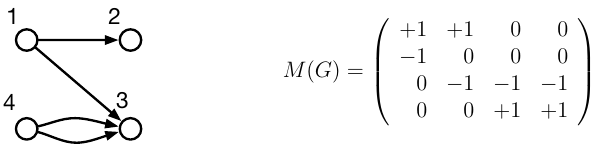
\includegraphics[width=0.8\textwidth, center]{./figures/incidence_matrix_dir.png}
                  \end{minipage}
                }
              }
              child {
                node {Degree
                  \resizebox{\textwidth}{!}{
                    \begin{minipage}[t]{12cm}
                      \begin{itemize}
                        \item the \alert{outdegree} $d^+(v)$ is the number of edges with tail $v$
                        \item the \alert{indegree} $d^-(v)$ is the number of edges with head $v$
                        \item the \alert{out-neighborhood (successor set)} $N^+(v) := \{x \in V(G) : v \rightarrow x\}$
                        \item the \alert{in-neighborhood (predecessor set)} $N^-(v) := \{x \in V(G) : x \rightarrow v\}$
                      \end{itemize}
                    \end{minipage}
                  }
                }
              }
            }
            child {
              node {Adjacency matrix $A(G)$
                \resizebox{\textwidth}{!}{
                  \begin{minipage}[t]{12cm}
                    \begin{itemize}
                      \item digraph $G$
                      \item the entry in position $a_{i,j}$ is the number of edges from $v_i$ to $v_j$
                    \end{itemize}
                    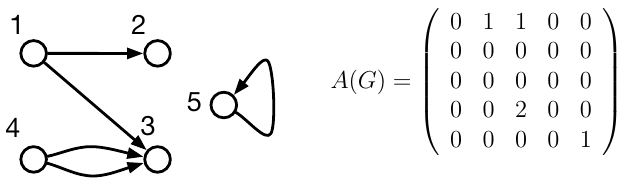
\includegraphics[width=0.8\textwidth, center]{./figures/adjacence_matrix_dir.png}
                  \end{minipage}
                }
              }
            }
          }
          child {
            node {Paths, Walks, Trails, Cycles, Circuits
              \resizebox{\textwidth}{!}{
                \begin{minipage}[t]{12cm}
                  \begin{itemize}
                    \item the \alert{length} is its \alert{number of edges}
                  \end{itemize}
                \end{minipage}
              }
            }
            child {
              node {Path (germ. Weg / Pfad)
                \resizebox{\textwidth}{!}{
                  \begin{minipage}[t]{12cm}
                    \begin{itemize}
                      \item a \alert{simple digraph} whose vertices can be linearly ordered so that: 
                        \begin{itemize}
                          \item there is an edge with tail $u$ and head $v$ \alert{iff} $v$ immediately follows $u$
                        \end{itemize}
                    \end{itemize}
                  \end{minipage}
                }
              }
              child {
                node {u,v-path (u,v-Pfad/-Weg)
                  \resizebox{\textwidth}{!}{
                    \begin{minipage}[t]{12cm}
                      \begin{itemize}
                        \item a path whose only vertex of \alert{indegree} $0$ is $u$ and \alert{outdegree} $0$ is $v$
                      \end{itemize}
                    \end{minipage}
                  }
                }
              }
              child {
                node {Cycle (germ. Kreis)
                  \resizebox{\textwidth}{!}{
                    \begin{minipage}[t]{12cm}
                      \begin{itemize}
                        \item a simple digraph whose vertices can be arranged on a circle such that: 
                          \begin{itemize}
                            \item edges exist \alert{iff} nodes follow each other according to the (without loss of generality) clockwise orientation
                          \end{itemize}
                      \end{itemize}
                    \end{minipage}
                  }
                }
              }
            }
            child {
              node {Walk (germ. Kantenzug)
                \resizebox{\textwidth}{!}{
                  \begin{minipage}[t]{12cm}
                    \begin{itemize}
                      \item a list $v_0, e_1, v_1, \ldots, e_k, v_k$ of vertices and edges
                        \begin{itemize}
                          \item for $1 \le i \le k$ the edge $e_i$ has tail (from) $v_{i-1}$ and head (to) $v_i$
                        \end{itemize}
                      \item trail and circuit (germ. Eulerzug) are the same in (undirected) graphs and digraphs, walk (germ. Kantenzug) is almost the same
                    \end{itemize}
                  \end{minipage}
                }
              }
              % child {
              %   node {Closed walk
              %     \resizebox{\textwidth}{!}{
              %       \begin{minipage}[t]{12cm}
              %         \begin{itemize}
              %           \item a walk with \alert{equal first} and \alert{last vertex}
              %         \end{itemize}
              %       \end{minipage}
              %     }
              %   }
              % }
              % child {
              %   node {Trail
              %     \resizebox{\textwidth}{!}{
              %       \begin{minipage}[t]{12cm}
              %         \begin{itemize}
              %           \item a walk \alert{without repeating edges}
              %         \end{itemize}
              %       \end{minipage}
              %     }
              %   }
              %   child {
              %     node {Circuit
              %       \resizebox{\textwidth}{!}{
              %         \begin{minipage}[t]{12cm}
              %           \begin{itemize}
              %             \item a \alert{closed trail}, i.e. the \alert{first} and the \alert{last vertex} are \alert{equal}
              %             \item like a circuit in computer engineering
              %           \end{itemize}
              %         \end{minipage}
              %       }
              %     }
              %   }
              % }
              % child {
              %   node {u,v-walk
              %     \resizebox{\textwidth}{!}{
              %       \begin{minipage}[t]{12cm}
              %         \begin{itemize}
              %           \item has \alert{first vertex} $u$ and \alert{last vertex} $v$
              %           % \item \alert a {walk} with \alert{first vertex} $u$ and \alert{last vertex} $v$
              %         \end{itemize}
              %       \end{minipage}
              %     }
              %   }
              % }
            }
          }
          child {
            node {(Strongly) Connected
              \resizebox{\textwidth}{!}{
                \begin{minipage}[t]{12cm}
                  \begin{itemize}
                    \item a digraph is \alert{weakly connected}
                      \begin{itemize}
                        \item if its underlying graph is connected
                      \end{itemize}
                    \item a digraph is \alert{strongly connected}
                      \begin{itemize}
                        \item if for each ordered pair $u$, $v$ there is a path from $u$ to $v$
                      \end{itemize}
                  \end{itemize}
                \end{minipage}
              }
            }
          }
        }
        child {
          node {(Undirected) Graphs $G = (V, E, R)$
            \resizebox{\textwidth}{!}{
              \begin{minipage}[t]{10cm}
                \begin{itemize}
                  \item \alert{vertex set}, e.g. $V(G) = \{v_1, v_2, \ldots\}$
                  \item \alert{edge set}, e.g. $E(G) = \{e_1, e_2, \ldots\}$
                  \item \alert{relation}, e.g. $R(G) = \{(e_1, \{v_1, v_2\}), \ldots\}$ that associates with each \alert{edge} a set of two vertices, called its \alert{endpoints}
                  \item a \alert{loop} is an edge with equal endpoints 
                  \item \alert{multiple edges} are edges with same pair of endpoints                       
                  \item \underline{\href[page=37]{\lpathgraph{Graphentheorie_english_all_in_one_with_go_back.pdf}}{interesting properties}:}
                    \begin{itemize}
                      \item if every vertex of a graph $G$ has degree at least $2$ then $G$ contains a cycle
                      \item $\displaystyle \sum_{v\in V(G)} d(v) = 2\cdot e(G)$
                      \item in a graph $G$ the average vertex degree is $\displaystyle \frac{\sum_{v\in V(G)} d(v)}{\mathrm{n}(\mathrm{G})}$ and hence $\displaystyle \delta(G) \leq \frac{2 \cdot e(G)}{n(G)} \leq \Delta(G)$
                      \item every graph has an even number of vertices of odd degree
                      \item a $k$-regular graph with $n$ vertices has $\dfrac{n\cdot k}{2}$ edges
                      \item the maximum number of edges in a simple graph is $\dbinom{n}{2}$
                      \item the minimum number of edges in a connected graph with $n$ vertices is $n-1$
                      \item if $G$ is a simple $n$-vertex graph with $\delta(G) \ge \dfrac{n-1}{2}$ then $G$ is connected
                    \end{itemize}
                \end{itemize}
              \end{minipage}
            }
          }
          child {
            node {Operations on Graphs}
            child {
              node (disjointunion) {Disjoint Union (germ. Disjunkte Vereinigung) $G+H$
                \resizebox{\textwidth}{!}{
                  \begin{minipage}[t]{12cm}
                    \begin{itemize}
                      \item for graphs $G$ and $H$ with disjoint sets of vertices is the union $(V(G) \cup V(H), E(G \cup E(H))$
                    \end{itemize}
                  \end{minipage}
                }
              }
            }
            child {
              node (join) {Join (germ. Join/Zusammenschluss) $G\vee H$
                \resizebox{\textwidth}{!}{
                  \begin{minipage}[t]{12cm}
                    \begin{itemize}
                      \item of simple graphs $G$ and $H$ is the graph obtained from the disjoint union $G+H$ by adding the edges $\{xy : x \in V(G), y \in V(H)\}$
                    \end{itemize}
                  \end{minipage}
                }
              }
            }
            child {
              node (cartesian) {Cartesian Product (germ. Kartesische Produkt) $G \square H$
                \resizebox{\textwidth}{!}{
                  \begin{minipage}[t]{12cm}
                    \resizebox{\textwidth}{!}{
                      \begin{minipage}[t]{12cm}
                        \begin{itemize}
                          \item the cartesian product of $G$ and $H$, is the graph with
                            \begin{itemize}
                              \item vertex set $V(G) \times V(H)$
                              \item $(u,v)$ is adjacent to $(u',v')$ \alert{iff} $u=u'$, $vv' \in E(H)$ or $v=v', uu' \in E(G)$
                            \end{itemize}
                          \item the cartesian operation is \alert{symmetric}: $G \square H \overset{\sim}{=} H\square G$
                          \item \href[page=218]{\lpathgraph{Graphentheorie_english_all_in_one_with_go_back.pdf}}{examples}
                        \end{itemize}
                      \end{minipage}
                    }
                  \end{minipage}
                }
              }
            }
            child {
              node (symmetricgraphdifference) {Symmetric Graph Difference
                \resizebox{\textwidth}{!}{
                  \begin{minipage}[t]{12cm}
                    \begin{itemize}
                      \item for graphs $G$ and $H$ with the same vertex set $V$ the \alert{symmetric difference $G \triangle H$} is the graph with vertex set $V$ whose edges are in $G$ or $H$, but not in both
                        \begin{itemize}
                          \item if $M$ and $M’$ are sets of edges in graphs $G$ und $H$, then we get as edge set: $M \triangle M’ = (M – M') \cup (M' – M)$
                        \end{itemize}
                    \end{itemize}
                  \end{minipage}
                }
              }
            }
          }
          child {
            node (connectivity) {Connectivity (germ. Zusammenhang)
              \resizebox{\textwidth}{!}{
                \begin{minipage}[t]{12cm}
                  \begin{itemize}
                    \item \alert{Theorem [Whiney]:} For simple graphs it applies that $\kappa(G) \le \kappa'(G) \le \delta(G)$
                      \begin{itemize}
                        \item $G = K_m + K_m$
                          \begin{itemize}
                            \item $\kappa(G) = \kappa’(G) = 0$
                            \item $\delta(G) = m-1$
                          \end{itemize}
                        \item $G$ is two $m$-cliques sharing a single vertex
                          \begin{itemize}
                            \item $\kappa(G) = 1$
                            \item $\kappa’(G) = \delta(G)$
                          \end{itemize}
                      \end{itemize}
                  \end{itemize}
                \end{minipage}
              }
            }
            child {
              node {(Vertex-) Connectivity
                \resizebox{\textwidth}{!}{
                  \begin{minipage}[t]{12cm}
                    \begin{itemize}
                      \item a \alert{separating set (germ. trennende Menge)} or \alert{vertex cut (germ. Knotenschnitt)} of a graph $G$ is a set $S \subseteq V(G)$ such that $G-S$ has more than one component
                      \item the \alert{connectivity (germ. Zusammenhang)} of $G$, \alert{$\kappa(G)$}, is the minimum size of $S \subseteq V(G)$ such that $G-S$ is disconnected or has only one vertex
                      \item a graph is \alert{k-connected (germ. k-zusammenhängend)} if its connectivity is at least $k$
                      \item a \alert{complete graph $K_n$} has connectivity $n-1$, i.e. $\kappa(K_n) = n − 2$
                        \begin{itemize}
                          \item $n-1$ vertex cut leaves only a single vertex after removal
                        \end{itemize}
                      \item for \alert{every non-complete graph} $G \ne K_n$ it applies that: $\kappa(G) \le n − 2$ 
                        \begin{itemize}
                          \item consider one vertex $v$ with at most $n-2$ neighbors 
                          \item the removal of the neighbors produces at least two components
                        \end{itemize}
                      \item for \alert{bipartite complete graphs} $\kappa(K_{n,m}) = min\{n, m\}$
                        \begin{itemize}
                          \item only the removal of the left or right bipartition cuts the graph
                        \end{itemize}
                    \end{itemize}
                  \end{minipage}
                }
              }
            }
            child {
              node (edgeconnectivity) {Edge-Connectivity
                \resizebox{\textwidth}{!}{
                  \begin{minipage}[t]{12cm}
                    \begin{itemize}
                      \item a \alert{disconnecting set of edges (germ. trennende Menge von Kanten)} is a set $F \subseteq E(G)$
                        \begin{itemize}
                          \item such that $G – F$ has more than one component
                        \end{itemize}
                      \item a graph is \alert{k-edge-connected (germ. $k$-kanten-zusammenhängend)}
                        \begin{itemize}
                          \item if every disconnected set of edges has at least $k$ edges
                        \end{itemize}
                      \item the \alert{edge-connectivity (germ. Kantenzusammenhang)} of $G, \kappa’(G)$,
                        \begin{itemize}
                          \item is the minimum size of a disconnecting set of edges
                        \end{itemize}
                      \item given $S, T \subseteq E[G]$ define $[S, T]$
                        \begin{itemize}
                          \item as the set of edges having one endpoint in $S$ and one endpoint in $T$
                        \end{itemize}
                      \item a \alert{edge cut (germ. Kantenschnitt)} is an edge set of the form $[S, \overline{S}]$ where $S \subsetneq V(G)$
                    \end{itemize}
                  \end{minipage}
                }
              }
            }
          }
          child {
            node {Matrix representation
              \resizebox{\textwidth}{!}{
                \begin{minipage}[t]{8cm}
                  \begin{itemize}
                    \item a \alert{loopless} graph $G$
                      \begin{itemize}
                        \item $V(G) = \{v_1, \ldots, v_n\}$
                        \item $E(G) = \{e_1, \ldots e_m\}$
                      \end{itemize}
                      used as example graph for the child nodes
                  \end{itemize}
                  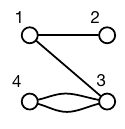
\includegraphics[width=0.3\textwidth, center]{./figures/matrix_representation.png}
                \end{minipage}
              }
            }
            child {
              node {Adjacency matrix $A(G)$
                \resizebox{\textwidth}{!}{
                  \begin{minipage}[t]{8cm}
                    \begin{itemize}
                      \item a $n\times n$ matrix with entries $a_{i,j}$
                      \item where $a_{i,j}$ is the number of edges with endpoints $\{v_i, v_j\}$
                    \end{itemize}
                    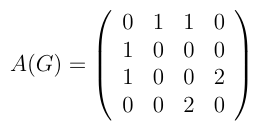
\includegraphics[width=0.3\textwidth, center]{./figures/adjacency_matrix.png}
                  \end{minipage}
                }
              }
              child {
                node {Adjacency
                  \resizebox{\textwidth}{!}{
                    \begin{minipage}[t]{8cm}
                      \begin{itemize}
                        \item if $u$ and $v$ are endpoints of an edge they are \alert{adjacent} and \alert{neighbors}
                        \item one writes: $u\leftrightarrow v$
                      \end{itemize}
                    \end{minipage}
                  }
                }
              }
            }
            child {
              node {Incidence matrix $M(G)$
                \resizebox{\textwidth}{!}{
                  \begin{minipage}[t]{8cm}
                    \begin{itemize}
                      \item a $n\times m$ matrix with entries $m_{i,j}$ (that means the $m$ columns are edges)
                      \item where $m_{i,j}$ is 
                        \begin{itemize}
                          \item $1$ if $v_i$ is an endpoint of $e_j$ and
                          \item $0$ otherwise
                        \end{itemize}
                    \end{itemize}
                    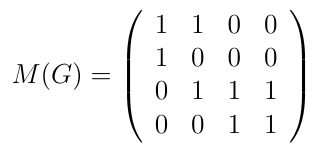
\includegraphics[width=0.3\textwidth, center]{./figures/incidence_matrix.png}
                  \end{minipage}
                }
              }
              child {
                node {Incidence
                  \resizebox{\textwidth}{!}{
                    \begin{minipage}[t]{8cm}
                      \begin{itemize}
                        \item $v$ and $e$ are \alert{incident} if $v$ is an endpoint of $e$
                      \end{itemize}
                    \end{minipage}
                  }
                }
                child {
                  node (degree) {Degree $d(v)$ or $d_G(v)$
                    \resizebox{\textwidth}{!}{
                      \begin{minipage}[t]{8cm}
                        \begin{itemize}
                          \item the \alert{degree} of vertex $v$ is the number of incident edges
                            \begin{itemize}
                              \item except for loops then the edge counts twice
                            \end{itemize}
                          \item \alert{maximum degree} is $\Delta(G)$
                          \item \alert{minimum degree} is $\delta(G)$
                          \item the number of $1$'s in a row of the incidence matrix
                        \end{itemize}
                      \end{minipage}
                    }
                  }
                }
              }
            }
          }
          child {
            % https://latex.org/forum/viewtopic.php?t=8650
            node {Complement $\overline{G}$
              \resizebox{\textwidth}{!}{
                \begin{minipage}[t]{8cm}
                  \begin{itemize}
                    \item of a simple graph $G$ is the simple graph with:
                      \begin{itemize}
                        \item vertex set $V(G)$
                        \item edge set $uv \in E(\overline{G}) \Leftrightarrow uv\not\in E(G)$
                      \end{itemize}
                  \end{itemize}
                \end{minipage}
              }
            }
          }
          child {
            node {Subgraph
              \resizebox{\textwidth}{!}{
                \begin{minipage}[t]{12cm}
                  \begin{itemize}
                    \item a \alert{subgraph }of a graph $G$ is a graph $H$ such that:
                      \begin{itemize}
                        \item $V(H)\subseteq V(G)$
                        \item $E(H)\subseteq E(G)$
                        \item the assignment of endpoints to edges in $H$ is the same as in $G$
                      \end{itemize}
                      % \item \href[page=29]{\lpathgraph{Graphentheorie_english_all_in_one_with_go_back.pdf}}{other definition for subgraph}
                    \item the \alert{subgraph $G - S$} is obtained by deleting a set of vertices $S$
                      \begin{itemize}
                        \item Edges are preserved \alert{iff} both endpoints are in $V(G)-S$
                      \end{itemize}
                    \item for $v \in V(G)$ let \alert{$G - v := G - \{v\}$}
                    \item the \alert{induced subgraph} $G[T] = G − \overline{T}$
                      \begin{itemize}
                        \item where $\overline{T} = V(G) − T$
                        \item is obtained by deleting all vertices of $\overline{T}$ while preserving all edges with both endpoints in $T$
                      \end{itemize}
                    \item $G − e$ denotes the graph, where the edge $e$ is removed but all vertices and other edges remain
                  \end{itemize}
                \end{minipage}
              }
            }
            child {
              node {Decomposition of a graph
                \resizebox{\textwidth}{!}{
                  \begin{minipage}[t]{8cm}
                    \begin{itemize}
                      \item germ. Kantenzerlegung (Dekomposition)
                      \item a \alert{list of subgraphs} such that \alert{a edge} appears in \alert{exactly one subgraph} in the list 
                    \end{itemize}
                  \end{minipage}
                }
              }
            }
          }
          child {
            node {Connected / Disconnected
              \resizebox{\textwidth}{!}{
                \begin{minipage}[t]{8cm}
                  \begin{itemize}
                    \item a graph $G$ is \alert{connected} if each pair of vertices in G belongs to a path
                    \item otherwise $G$ is \alert{disconnected}
                  \end{itemize}
                \end{minipage}
              }
            }
            child {
              node {Components
                \resizebox{\textwidth}{!}{
                  \begin{minipage}[t]{12cm}
                    \begin{itemize}
                      \item the (connected) \alert{components} of a graph $G$ are its maximal connected subgraphs
                      \item a component is \alert{trivial} if it has no edges
                      \item an \alert{isolated} vertex is a vertex of degree $0$
                      \item every graph with $n$ vertices and k edges has at least $n-k$ components
                    \end{itemize}
                  \end{minipage}
                }
              }
              child {
                node {Cut-edge
                  \resizebox{\textwidth}{!}{
                    \begin{minipage}[t]{12cm}
                      \begin{itemize}
                        \item an edge whose deletion increases the number of components
                          \begin{itemize}
                            \item an edge is a cut-edge if and only if it belongs to no cycle
                          \end{itemize}
                      \end{itemize}
                    \end{minipage}
                  }
                }
              }
              child {
                node {Cut-vertex
                  \resizebox{\textwidth}{!}{
                    \begin{minipage}[t]{12cm}
                      \begin{itemize}
                        \item a vertex whose deletion increases the number of components
                      \end{itemize}
                    \end{minipage}
                  }
                }
                child {
                  node {Blocks
                    \resizebox{\textwidth}{!}{
                      \begin{minipage}[t]{12cm}
                        \begin{itemize}
                          \item A \alert{block of a graph} G is a \alert{maximal connected subgraph} of G that has \alert{no cut-vertex}
                          \item If G itself is \alert{connected} and has \alert{no cut-vertex}, then G is a \alert{block}
                          \item If a block has more than two vertices then it is $2$-connected
                          \item If $H$ is a block of $G$, then $H$ as a graph has no cut-vertex, but $H$ may contain vertices that are cut-vertices of $G$
                          \item a node $u$ is a cut-vertex \alert{iff} there is \alert{no backward edge} from a descendant of $u$ to an ancestor of $u$ in the DFS tree B
                          \item \href[page=111]{\lpathgraph{Graphentheorie_all_in_one_with_go_back.pdf}}{algorithm}
                          \item \href[page=112]{\lpathgraph{Graphentheorie_all_in_one_with_go_back.pdf}}{block-cutpoint graph}
                            % \item Ein Knoten u ist genau dann ein Schnittknoten, wenn es im DFS-Baum keine Rückwärtskante von den Nachfolgern in B von u zu seinem Vorgängern im Baum B gibt.
                        \end{itemize}
                      \end{minipage}
                    }
                  }
                }
              }
            }
          }
          child {
            node {Paths, Walks, Trails, Cycles, Circuits
              \resizebox{\textwidth}{!}{
                \begin{minipage}[t]{12cm}
                  \begin{itemize}
                    \item the \alert{length} is its \alert{number of edges}
                  \end{itemize}
                \end{minipage}
              }
            }
            child {
              node {Walk (germ. Kantenzug)
                \resizebox{\textwidth}{!}{
                  \begin{minipage}[t]{8cm}
                    \begin{itemize}
                      \item a list $v_0, e_1, v_1, \ldots, e_k, v_k$ of \alert{vertices} and \alert{edges}
                        \begin{itemize}
                          \item for $1 \le i \le k$ the \alert{edge} $e_i$ has \alert{endpoints} $v_{i-1}$ and $v_i$
                        \end{itemize}
                      \item a \enquote{\alert{walk $W$ contains a path $P$}} if the vertices and edges of $P$ occur as a sublist of the vertices and edges of $W$
                    \end{itemize}
                  \end{minipage}
                }
              }
              child {
                node {u,v-walk (germ. u,v-Kantenzug)
                  \resizebox{\textwidth}{!}{
                    \begin{minipage}[t]{8cm}
                      \begin{itemize}
                        \item a \alert{walk} with \alert{first vertex} $u$ and \alert{last vertex} $v$
                      \end{itemize}
                    \end{minipage}
                  }
                }
              }
              child {
                node {Closed walk (germ. Zyklus / geschlossener Kantenzug)
                  \resizebox{\textwidth}{!}{
                    \begin{minipage}[t]{8cm}
                      \begin{itemize}
                        \item a walk with \alert{equal first} and \alert{last vertex}
                      \end{itemize}
                    \end{minipage}
                  }
                }
              }
              child {
                node {Trail
                  \resizebox{\textwidth}{!}{
                    \begin{minipage}[t]{8cm}
                      \begin{itemize}
                        \item a walk \alert{without repeating edges}
                      \end{itemize}
                    \end{minipage}
                  }
                }
                child {
                  node {Circuit
                    \resizebox{\textwidth}{!}{
                      \begin{minipage}[t]{12cm}
                        \begin{itemize}
                          \item a \alert{closed trail}, i.e. the \alert{first} and the \alert{last vertex} are \alert{equal}
                        \end{itemize}
                      \end{minipage}
                    }
                  }
                }
              }
            }
            child {
              node {Path (germ. Weg/Pfad)
                \resizebox{\textwidth}{!}{
                  \begin{minipage}[t]{8cm}
                    \begin{itemize}
                      \item a \alert{simple graph} whose vertices can be ordered such that:
                        \begin{itemize}
                          \item two vertices are adjacent \alert{iff} they are consecutive in the list
                        \end{itemize}
                    \end{itemize}
                    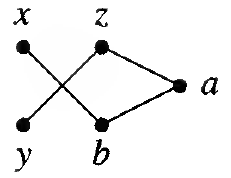
\includegraphics[width=0.3\textwidth, center]{./figures/path.png}
                  \end{minipage}
                }
              }
              child {
                node {u,v-path (germ. u,v-Pfad/-Weg)
                  \resizebox{\textwidth}{!}{
                    \begin{minipage}[t]{8cm}
                      \begin{itemize}
                        \item a path whose vertices of \alert{degree} $1$ are $u$ and $v$ if $u\ne v$
                        \item if $u=v$ then the $u,v$-path consists only of vertex $u$ and has no edges
                      \end{itemize}
                    \end{minipage}
                  }
                }
              }
              child {
                node {Cycle (germ. Kreis)
                  \resizebox{\textwidth}{!}{
                    \begin{minipage}[t]{8cm}
                      \begin{itemize}
                        \item a simple graph
                          \begin{enumerate}
                            \item with an \alert{equal} number of \alert{vertices} and \alert{edges}
                            \item whose \alert{vertices} can be placed around a \alert{circle} such that:
                              \begin{itemize}
                                \item two vertices are adjacent \alert{iff} they are consecutive in the circle
                              \end{itemize}
                          \end{enumerate}
                      \end{itemize}
                      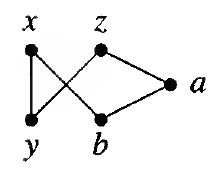
\includegraphics[width=0.3\textwidth, center]{./figures/cycle.png}
                    \end{minipage}
                  }
                }
              }
            }
          }
          child {
            node {Isomorphism
              \resizebox{\textwidth}{!}{
                \begin{minipage}[t]{8cm}
                  \begin{itemize}
                    \item an \alert{isomorphism} from a \alert{simple graph} $G$ to a \alert{simple graph} $H$ is a \alert{bijection} $f: V(G) \rightarrow V(H)$ such that
                      \begin{itemize}
                        \item $uv\in E(G)$ \alert{iff} $f(u)f(v)\in E(H)$
                      \end{itemize}
                    \item one says \enquote{\alert{$G$ is isomorphic to $H$}} if there is an \alert{isomorphism} from $G$ to $H$ 
                    \item one writes: $G \cong H$
                  \end{itemize}
                \end{minipage}
              }
            }
          }
        };
      \end{scope}
      % ┌───────────────────┐
      % │ Verbindungslinien │
      % └───────────────────┘
      \begin{pgfonlayer}{background}
        \draw [concept connection]
        %     (commoncasefast) edge (amdahl)
        %     (branchpredictionbuffer) edge (2bitpredictor)
        %     (loadusedatahazard) edge (forwarding)
        (bipartite graphs) edge (independant set)
        (disjointunion) edge (coloring)
        (join) edge (coloring)
        (cartesian) edge (coloring)
        (vc) edge (isvccqcl)
        (clique) edge (isvccqcl)
        (coloring) edge (isvccqcl)
        (vc) edge (apa)
        (regular graphs) edge (degree)
        (gt) edge (degree)
        (symmetricdifferencematching) edge (symmetricgraphdifference)
        (connectivity) edge (hypercube)
        (edgecut) edge (edgeconnectivity)
        (edgecut) edge (cut)
        (ec) edge (mec);
      \end{pgfonlayer}
      % ┌──────────────┐
      % │ Annotationen │
      % └──────────────┘
      % https://tex.stackexchange.com/questions/302976/node-positioning-middle-point-mind-map-connection-bar
      \node [annotation, below] at (gt.south) {This mindmap is provided without guarantee of correctness and completeness!};
      \node [annotation, below] at (gt.north) {\href{https://www.youtube.com/playlist?list=PLmsC317bB1b0m9-ZCKGNR6iM6UTPUO__r}{Recordings} where the different topics of this mindmap get explained\\\href{/tmp/current.pdf}{go back}};
      % \path (measuringexecutiontime) -- node[annotation, above, align=center, pos=0.01] {Similiar to \textbf{Response Time:} How long it takes to do a task} (ca);
      % \path (performance) -- node[annotation, above, align=center, pos=0.01] {Similiar to \textbf{Throughput}: Total work done per time unit (e.g. tasks, transactions\ldots / per hour)} (ca);
      % \path (elapsedtime) -- node[annotation, above, align=center, pos=0.01] {Also called \textbf{Wall Clock Time} or \textbf{Real Time}} (ca);
      % \path (cputime) -- node[annotation, above, align=center, pos=0.01] {Also called \textbf{User Time}} (ca);
      % % \path (branchpredictionbuffer) -- node[annotation, below, align=center, pos=-0.06] {Also called Branch History Table} (ca);
      % \path (multicycle) -- node[annotation, above, align=center, pos=0.01] {Optimize space} (ca);
      % \path (pipelining) -- node[annotation, above, align=center, pos=0.01] {Optimize time} (ca);
    \end{tikzpicture}
    \end{document}
